\documentclass[JEP,XML,SOM,Unicode, NoEqCountersInSection,NoFloatCountersInSection,published]{cedram}
\datereceived{2020-05-30}
\dateaccepted{2022-02-11}
\dateepreuves{2022-02-15}

\newenvironment{enumeratei}
{\bgroup\def\theenumi{\roman{enumi}}\def\theenumii{\arabic{enumii}}\begin{enumerate}}
{\end{enumerate}\egroup}
\newenvironment{enumeratea}
{\bgroup\def\theenumi{\alph{enumi}}\begin{enumerate}}
{\end{enumerate}\egroup}

\AtBeginDocument{%
\renewcommand\labelitemi{$\scriptscriptstyle\bullet$}%
}
\newcommand{\Psfrac}[2]{(\sfrac{#1}{#2})}
\newcommand{\psfrac}[2]{\sfrac{(#1)}{#2}}
\newcommand{\spfrac}[2]{\sfrac{#1}{(#2)}}

\usepackage{graphicx}
\graphicspath{{humbert-et-al_fig/}}

\def\R{\mathbb{R}}
\def\N{\mathbb{N}}
\def\Z{\mathbb{Z}}

\newcommand{\CC}{\mathbb{C}}\let\C\CC

\newcommand{\Op}{\mathrm{Op}}

\newtheorem{theorem}{Theorem}
\newtheorem*{thmnonumbering}{Theorem}
\newtheorem{step}{Step}
\newtheorem{proposition}{Proposition}
\newtheorem{corollary}{Corollary}
\newtheorem{lemma}{Lemma}
\theoremstyle{definition}
\newtheorem{remark}{Remark}
\newtheorem{example}{Example}
\newtheorem{definition}{Definition}

\datepublished{2022-02-16}
\begin{document}

\title{Geometric and probabilistic results for the~observability of the wave equation}
\alttitle{Résultats géométriques et probabilistes pour l'observabilité de l'équation des ondes}

\author[\initial{E.} \lastname{Humbert}]{\firstname{Emmanuel} \lastname{Humbert}}
\address{Institut Denis Poisson, UFR Sciences et Technologie, Faculté François Rabelais\\
Parc de Grandmont, 37200 Tours, France}
\email{emmanuel.humbert@lmpt.univ-tours.fr}
\urladdr{http://www.lmpt.univ-tours.fr/~humbert/}

\author[\initial{Y.} \lastname{Privat}]{\firstname{Yannick} \lastname{Privat}}
\address{IRMA, Université de Strasbourg, CNRS UMR 7501\\
7 rue René Descartes, 67084 Strasbourg, France\\
\& Institut Universitaire de France (IUF)}
\email{yannick.privat@unistra.fr}
\urladdr{https://irma.math.unistra.fr/~privat/}

\author[\initial{E.} \lastname{Trélat}]{\firstname{Emmanuel} \lastname{Trélat}}
\address{Sorbonne Université, CNRS, Université de Paris, Inria, Laboratoire Jacques-Louis Lions (LJLL)\\
F-75005 Paris, France}
\email{emmanuel.trelat@sorbonne-universite.fr}
\urladdr{https://www.ljll.math.upmc.fr/trelat/}

\begin{abstract}
Given any measurable subset $\omega$ of a closed Riemannian manifold and given any $T>0$, we define $\ell^T(\omega)\in[0,1]$ as the smallest average time over $[0,T]$ spent by all geodesic rays in $\omega$. Our first main result, which is of geometric nature, states that, under regularity assumptions, $1/2$ is the maximal possible discrepancy of $\ell^T$ when taking the closure. Our second main result is of probabilistic nature: considering a regular checkerboard on the flat two-dimensional torus made of $n^2$ square white cells, constructing random subsets $\omega_\varepsilon^n$ by darkening cells randomly with a probability $\varepsilon$, we prove that the random law $\ell^T(\omega_\varepsilon^n)$ converges in probability to~$\varepsilon$ as $n\rightarrow+\infty$. We discuss the consequences in terms of observability of the wave equation.
\end{abstract}

\begin{altabstract}
Étant donné un sous-ensemble mesurable $\omega$ d'une variété riemannienne compacte et étant donné $T>0$, on définit $\ell^T(\omega)\in[0,1]$ comme étant le plus petit temps moyen passé par les rayons géodésiques dans $\omega$. Notre premier résultat principal, qui est de nature géométrique, établit que, sous des conditions de régularité, $\ell^T$ peut augmenter au maximum de $1/2$ en passant à l'adhérence. Notre second résultat principal est de nature probabiliste: considérant un damier régulier sur le tore plat de dimension $2$ formé de $n^2$ carrés blancs, construisant des ensembles aléatoires $\omega_\varepsilon^n$ en noircissant les carrés de manière aléatoire avec probabilité $\varepsilon$, on~montre que la variable aléatoire $\ell^T(\omega_\varepsilon^n)$ converge en probabilité vers $\varepsilon$ lorsque $n\rightarrow+\infty$. Nous discutons les conséquences en termes d'observabilité de l'équation des ondes.
\end{altabstract}

\subjclass{93B07, 53C22, 60B10}

\keywords{Observability, wave equation, Riemannian geometry, random set}

\altkeywords{Observabilité, équation des ondes, géométrie riemannienne, ensemble aléatoire}

\maketitle
\vspace*{-\baselineskip}\enlargethispage{\baselineskip}%
\tableofcontents


\vspace*{-3.5\baselineskip}\mbox{ }
\section{Introduction and main results}\label{sec1}
Let $(M,g)$ be a closed connected Riemannian manifold.
We denote by $\Gamma$ the set of geodesic rays, that is, the set of projections onto $M$ of Riemannian geodesic curves in the co-sphere bundle $S^*M$.
Given any $T>0$ and any Lebesgue measurable subset $\omega$ of $M$, we define\vspace*{-3pt}
\begin{equation}\label{defg2}
\ell^T(\omega) = \inf_{\gamma\in\Gamma} \frac{1}{T} \int_0^T \chi_\omega(\gamma(t)) \, dt.
\end{equation}
Here, $\chi_\omega$ is the characteristic function of $\omega$, defined by $\chi_\omega(x)=1$ if $x\in\omega$ and $\chi_\omega(x)=0$ if $x\in M\setminus\omega$.
The real number $\ell^T(\omega)\in[0,1]$ is the smallest average time over $[0,T]$ spent by all geodesic rays in $\omega$.
This quantity appears naturally when studying observability properties for the wave equation on $M$ with $\omega$ as an observation subset.

In this article we establish two properties of the functional $\ell^T$, one is geometric and the other is probabilistic. Let us describe them in few words.

The first geometric property is on the maximal discrepancy of $\ell^T$ when taking the closure. We may have $\ell^T(\mathring{\omega})<\ell^T(\overline\omega)$ whenever there exist rays grazing $\omega$ and the discrepancy between both quantities may be equal to $1$ for some subsets $\omega$. We prove that, if the metric $g$ is $C^2$ and if $\omega$ satisfies a slight regularity assumption, then $\ell^T(\overline\omega) \leq \frac{1}{2} \left( \ell^T(\mathring{\omega}) + 1 \right)$.
We also show that our assumptions are essentially sharp; in~particular, surprisingly the result is wrong if the metric $g$ is not $C^2$.
As a consequence, if $\omega$ is regular enough and if $\ell^T(\overline\omega)>1/2$ then the Geometric Control Condition is satisfied and thus the wave equation is observable on $\omega$ in time $T$.

The second property is of probabilistic nature. We take $M=\mathbb{T}^2$, the flat two-dimensional torus, and we consider a regular grid on it, a regular checkerboard made of $n^2$ square white cells. We construct random subsets $\omega_\varepsilon^n$ by darkening each cell in this grid with a probability $\varepsilon$. We prove that the random law $\ell^T(\omega_\varepsilon^n)$ converges in probability to $\varepsilon$ as $n\rightarrow+\infty$.
As a consequence, if $n$ is large enough then the Geometric Control Condition is satisfied almost surely and thus the wave equation is observable on $\omega_\varepsilon^n$ in time $T$.

\subsubsection*{Observability and Geometric Control Condition.}
The condition
\[
\ell^T(\omega)>0
\]
means that all geodesic rays, propagating in $M$, meet $\omega$ within time $T$. This condition, usually called \textit{Geometric Control Condition} (in short, GCC), is related to observability properties for the wave equation
\begin{equation}\label{waveEqobs}
\partial_{tt}y- \triangle_g y=0\qquad \textrm{in }(0,T)\times M,
\end{equation}
where $\triangle_g$ is the Laplace-Beltrami operator on $M$ for the metric $g$.
More precisely, denoting by $dx_g$ the canonical Riemannian volume, we define the observability constant $C_T(\omega)\geq 0$ as the largest possible nonnegative constant $C$ such that the inequality
\begin{equation} \label{ineqobsw}
\int_0^T \int_\omega |y(t,x)|^2 \, dx_g \, dt \geq C \Bigl( \Vert y(0,\cdot)\Vert_{L^2(M)}^2 + \Vert\partial_t y(0,x)\Vert_{H^{-1}(M)}^2 \Bigr)
\end{equation}
is satisfied for any solution $y$ of \eqref{waveEqobs}, that is,
\[
C_T(\omega) = \inf \biggl\{ \int_0^T \int_\omega | y(t,x)|^2 \, dx_g \, dt \mid \Vert (y(0,\cdot),\partial_t y(0,\cdot))\Vert_{L^2(M)\times H^{-1}(M)}=1 \biggr\}.
\]
When $C_T(\omega)>0$, the wave equation \eqref{waveEqobs} is said to be \textit{observable} on $\omega$ in time $T$, and when $C_T(\omega)=0$ we say that observability does not hold for $(\omega,T)$.

It has been proved in \cite{BardosLebeauRauch,rauch-taylor} that, for $\omega$ open, observability holds if the pair $(\omega,T)$ satisfies GCC, \ie if $\ell^T(\omega)>0$.
In other words, if $\omega$ is open and satisfies $\ell^T(\omega)>0$ then the wave equation \eqref{waveEqobs} is observable on $\omega$ in time $T$.

The converse is not true: GCC is not a necessary condition for observability.
It~is shown in \cite{Lebeau_JEDP1992} that, if $M=\mathbb{S}^2$ (the unit sphere in $\R^3$ endowed with the restriction of the Euclidean structure), if $\omega$ is the open Northern hemisphere, then $\ell^T(\omega)=0$ for every $T>0$, and however one has $C_T(\omega)>0$ for every $T>\pi$. The latter fact is established by an explicit computation exploiting symmetries of solutions.
This failure of the functional $\ell^T$ to capture the observability property is due, here, to the existence of a very particular geodesic ray which is \emph{grazing} the open set $\omega$, namely, the equator.
In this example, considering the closure $\overline\omega$ of $\omega$, it is interesting to observe that $\ell^T(\overline\omega)=0$ for every $T\leq\pi$ (take a geodesic ray contained in the closed Southern hemisphere) and $\ell^T(\overline\omega)>0$ for every $T>\pi$, with $\ell^T(\overline\omega)=\frac{1}{2}$ when $T\geq 2\pi$. The latter equality is in contrast with $\ell^T(\omega)=0$: there is thus a discrepancy $1/2$ in the value of~$\ell^T$ for $T\geq 2\pi$ when taking the closure of $\omega$. In this specific case, this discrepancy is caused by the equator, which is a geodesic ray grazing the open subset $\omega$.

Our first main result below shows that $1/2$ is actually the maximal possible discrepancy.

\subsection{A geometric result on the maximal discrepancy of $\ell^T$}
In general, one can always find subsets $\omega$ for which the difference $\ell^T(\overline\omega)- \ell^T(\mathring{\omega})$ is arbitrary close to~$1$. Surprisingly, under slight regularity assumptions, this maximal discrepancy is~$1/2$ only.

\begin{theorem} \label{thm_geom}
Let $T>0$ be arbitrary and let $\omega$ be a measurable subset of~$M$.
We~make the following assumptions:
\begin{enumeratei}
\item\label{thm_geomi}
The metric $g$ is at least of class $C^2$.
\item\label{thm_geomii}
$\omega$ is an embedded $C^1$ submanifold of $M$ with boundary if $\dim M \geq 3$ and is piecewise $C^1$ if $\dim M=2$.
\end{enumeratei}
Then
\begin{equation}\label{mainineq}
\ell^T(\overline\omega) \leq \frac{1}{2}\bigl( \ell^T(\mathring{\omega}) + 1\bigr).
\end{equation}
\end{theorem}

We give more details and a number of comments on this theorem in Section \ref{sec_geom}. At the opposite, as an obvious remark, if there is no geodesic ray {grazing} $\omega$ then $\ell^T(\overline\omega)=\ell^T(\mathring{\omega})$. {Here and throughout the paper, we say that a geodesic ray $\gamma$ is grazing $\omega$ if $\int_0^T\chi_{\partial\omega}(\gamma(t))\, dt>0$, where $\partial\omega=\overline\omega\setminus\mathring{\omega}$.}

In more general, the existence of grazing rays adds a serious difficulty to the analysis of observability (see \cite{BardosLebeauRauch}). It is noticeable that, if one replaces the characteristic function~$\chi_\omega$ of $\omega$ by a continuous function $a$, in the integral at the left-hand side of~\eqref{ineqobsw} (\ie $\int_0^T\int_M a(x)\vert y(t,x)\vert^2\, dx_g\, dt$) as well as in the definition \eqref{defg2} of the functional $\ell^T$, this difficulty disappears and the condition $\ell^T(a)>0$ becomes a necessary and sufficient condition for observability of~\eqref{waveEqobs} on $\omega$ in time $T$ (see \cite{BurqGerard1997}).

By the way, for completeness, we provide in the appendix some semi-continuity properties of the functional $\ell^T$, which may be of interest for other purposes.

The issue of the observability on a general measurable subset $\omega\subset M$ has remained widely open for a long time. Recent advances have been made, which we can summarize as follows. It has been established in \cite{hpt} that observability on a measurable subset~$\omega$ in time $T$ is satisfied if and only if $\alpha_T(\omega)>0$. The quantity $\alpha_T(\omega)$, defined in~\cite{hpt} as the limit of high-frequency observability constants, is however not easy to compute and we have, in general, the inequality $\ell^T(\mathring{\omega}) \leq \alpha_T(\omega) \leq \ell^T(\overline\omega)$. In particular, the condition $\ell^T(\omega)>0$ becomes a necessary and sufficient condition for observability as soon as there are no geodesic rays grazing $\omega$.
It has also been shown in \cite{hpt} that $\lim_{T \to+ \infty}\sfrac{C_T(\omega)}{T}$ is the minimum of two quantities, one of them being $\ell^T(\overline\omega)$ and the other being of a spectral nature.

We have the following corollary of Theorem \ref{thm_geom}, using the fact that, since $\mathring{\omega}$ is open, the condition $\ell^T(\mathring{\omega})>0$ implies observability for $(\mathring{\omega},T)$, and thus $C_T(\omega)\geq C_T(\mathring{\omega})>0$.

\begin{corollary} \label{cor_geom}
Under the assumptions of Theorem \ref{thm_geom}, if $\ell^T(\overline\omega) >1/2$ then $\ell^T(\mathring{\omega})>0$ and thus the wave equation \eqref{waveEqobs} is observable on $\omega$ in time $T$, \ie $C_T(\omega)>0$.
\end{corollary}

Note that Corollary \ref{cor_geom} does not apply to the (limit) case where $M=\mathbb{S}^2$ and $\omega$ is the open Northern hemisphere. It does neither apply to the case where $M$ is the two-dimensional torus and $\omega$ is a half-covering open checkerboard on it, as in \cite{Burq2017,BurqGerard2018} (see next section). Indeed, in these two cases, we have $\ell^T(\omega)=0$ for every $T>0$ but $C_T(\omega)>0$ (\ie we have observability) for $T$ large enough. This is due to the fact that trapped rays are the weak limit of Gaussian beams that oscillate \emph{on both sides} of the limit ray, spreading on one side and on the other a sufficient amount of energy so that indeed observability holds true. In full generality, having information on the way that semi-classical measures, supported on a grazing ray, can be approached by high-frequency wave packets such as Gaussian beams, is a difficult question. In the case of the sphere, symmetry arguments give the answer (see \cite{Lebeau_JEDP1992}). In the case of the torus, a much more involved analysis is required, based on second microlocalization arguments (see \cite{Burq2017,BurqGerard2018}).

Anyway, Corollary \ref{cor_geom} can as well be applied for instance to any kind of checkerboard domain $\omega$ on the two-dimensional torus, as soon as the measure of $\omega$ is large enough so that $\ell^T(\overline\omega)>1/2$.

Since the case of checkerboards (in dimension two) is interesting and challenging, following a question by Nicolas Burq, in the next section we investigate the case of random checkerboards on the flat torus and we establish our second main result.

\Subsection{A probabilistic result for random checkerboards on the flat torus}
In this section, we take $M=\mathbb{T}^2= \R^2/ \Z^2$ (flat torus) which is identified to the square $[0,1]^2$, class of equivalence of $\R^2$ under the identifications $(x,y)\sim(x+1,y)\sim(x,y+1)$, inheriting of the Euclidean metric.
Given any subset $A$ of $M$, we denote by~$|A|$ the (two-dimensional) Lebesgue measure of $A$.

We consider a regular grid $\mathcal{G}^n= (c_{ij}^n)_{1 \leq i,j \leq n}$ in the square, like a checkerboard, made of $n \times n$ closed squares:
\[
[0,1]^2 = \bigcup_{i,j=1}^n c_{ij}^n\quad\textrm{with}\quad c_{ij}^n = [(i-1)/n,i/n]\times[(j-1)/n,j/n]\quad \forall (i,j)\in\{1,\ldots,n\}^2.
\]
Defining $c_{i'j'}$ in the same way for all $(i',j') \in \Z^2$, we identify the square $c_{i'j'}$ to the square $c_{ij}^n$ of the above grid with $(i,j)\in \{1,\ldots,n\}^2$ such that $i = i'\mod n$ and $j= j'\mod n$.

\subsubsection*{Construction of random checkerboards.}
Let $\varepsilon \in [0, 1]$ be arbitrary.
Considering that all squares in the grid are initially white, we construct a random checkerboard by randomly darkening some squares in the checkerboard as follows: for every $(i,j)\in \{1,\ldots,n\}^2$, we darken the square $c_{ij}^n$ of the grid with a probability $\varepsilon$. All choices are assumed to be mutually independent.
In other words, we make a selection of squares (that are paint in black) in the grid by considering $n^2$ independent Bernoulli random variables denoted $(X_{ij}^n)_{1\leq i,j\leq n}$, each of them with parameter $\varepsilon$.
The total number of black squares follows therefore the binomial law $B(n^2,\varepsilon)$.

We denote by $\omega_\varepsilon^n$ the resulting closed subset of $[0,1]^2$ that is the union of all {(closed)} black squares (see Figure \ref{fig_checkerboard}).
\begin{figure}[htb]
\begin{center}
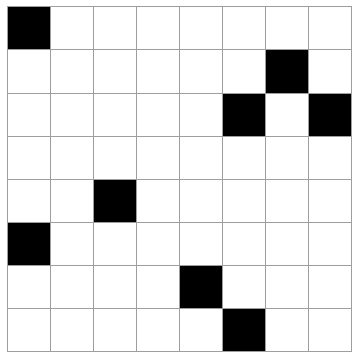
\includegraphics[width=2.8cm]{checkerboard1.png}\qquad
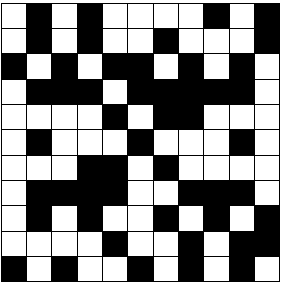
\includegraphics[width=2.8cm]{checkerboard2.png}\\[5mm]
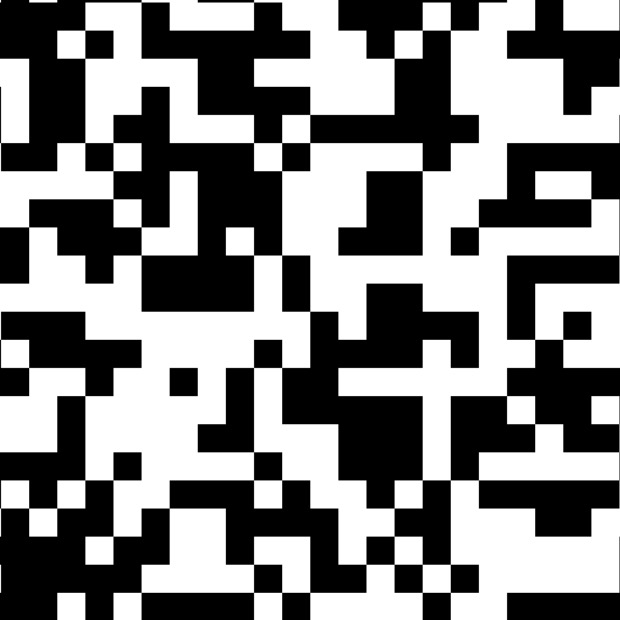
\includegraphics[width=2.8cm]{checkerboard3.jpg}\qquad
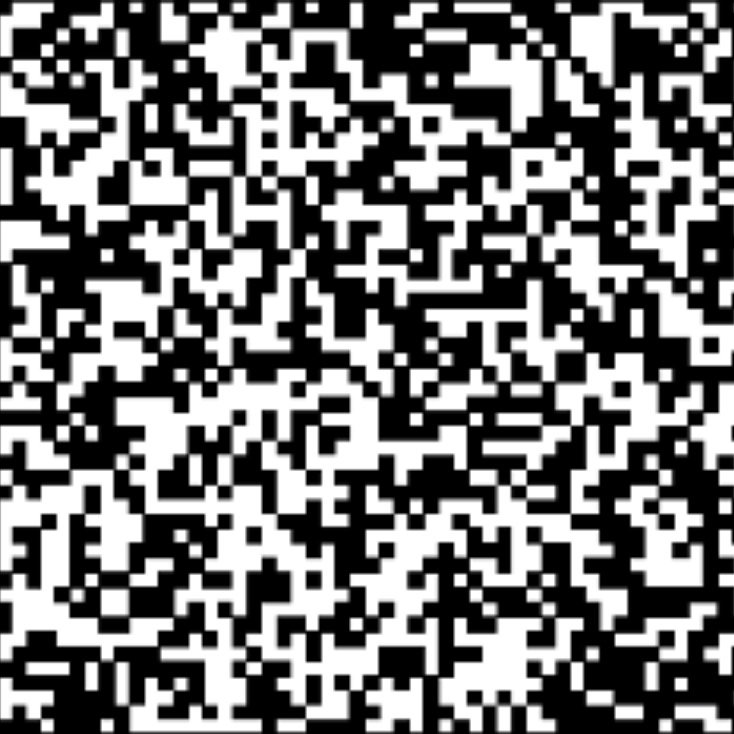
\includegraphics[width=2.8cm]{checkerboard4.jpg}
\end{center}
\caption{Some examples of random checkerboards. The random {(closed)} subset $\omega_\varepsilon^n\subset[0,1]^2$ is the union of {(closed)} black squares.\label{fig_checkerboard}}
\end{figure}

Given any fixed $T>0$ and $\varepsilon\in(0,1]$, our objective is to understand how well the random set $\omega_\varepsilon^n$ is able to capture all geodesic rays propagating in $M\simeq[0,1]^2$, in finite time $T$. In other words, we want to study the random variable $\ell^T(\omega_\varepsilon^n)$. Of course, the random variable $\vert\omega_\varepsilon^n\vert$ follows the law $\Psfrac{1}{n^2}B(n^2,\varepsilon)$ and thus its expectation is equal to $\varepsilon$, and so, when $\varepsilon$ is small, $\omega_\varepsilon^n$ covers only a small area in $[0,1]^2$. And yet, our second main result below shows that, for $n$ large, almost all such random sets meet all geodesic rays within time $T$.

\begin{theorem}\label{thm_random}
Given any $T>0$ and any $ \varepsilon \in [0, 1]$, the random variable $\ell^T(\omega_\varepsilon^n)$ converges in probability to $\varepsilon$ as $n\to +\infty$, \ie
\[
\lim_{n\to +\infty}\mathbb{P}\left(\vert\ell^T(\omega_\varepsilon^n) - \varepsilon \vert \geq \delta\right) = 0 \qquad \forall \delta>0.
\]
\end{theorem}

Theorem \ref{thm_random} is proved in Section \ref{sec_random}. As mentioned above, this issue has emerged following a question by Nicolas Burq.
In \cite{Burq2017,BurqGerard2018}, the authors also consider checkerboard domains, as above, but not in a random framework. As a consequence of their analysis, given any $T>0$, any $\varepsilon\in[0,1]$ and any $n\in\N^*$ fixed, if all geodesic rays of length~$T$, either meet the interior of $\omega_\varepsilon^n$ (\ie the interior of some black square), or follow for some positive time one of the sides of a black square on the left and for some positive time one of the sides of a black square (possibly the same) on the right, then $C_T(\omega_\varepsilon^n)>0$, \ie the wave equation on the torus $M=\mathbb{T}^2$ is observable on $\omega_\varepsilon^n$ in time~$T$.

Let $T>0$ and let $\varepsilon \in(0,1]$ be arbitrary. According to Theorem \ref{thm_random}, for $n$ large enough, almost every subset $\omega_\varepsilon^n$ (constructed randomly as above) is such that $\ell^T(\omega_\varepsilon^n)>0$. This implies that every geodesic ray, that is neither horizontal nor vertical, meets the interior of $\omega_\varepsilon^n$ within time $T$, and that every horizontal or vertical geodesic ray meets the closed subset $\omega_\varepsilon^n$ within time $T$ (for some positive time, not less than $\ell^T(\omega_\varepsilon^n)$). In the latter case, moreover, by construction of the random set~$\omega_\varepsilon^n$, the probability that vertical grazing rays follow for some positive time one of the sides of a black square on the left and for some positive time one of the sides of a black square on the right, converges to $1$ as $n\rightarrow +\infty$.

All in all, combining Theorem \ref{thm_random}, the result of \cite{Burq2017,BurqGerard2018} and the above reasoning, we have the following consequence in terms of observability of the wave equation.

\begin{corollary}
Given any $T>0$ and $\varepsilon \in(0,1]$, may they be arbitrarily small, the probability that the wave equation on the torus $M=\mathbb{T}^2$ be observable on $\omega_\varepsilon^n$ in time~$T$ tends to $1$ as $n\rightarrow+\infty$.
\end{corollary}

In other words, observability in (any) finite time is almost surely true for large $n$, despite the fact that the measure of $\omega_\varepsilon^n$ may be very small!

Note that, for $\varepsilon>1/2$, almost sure observability follows from Corollary \ref{cor_geom} (indeed, the random sets constructed above are piecewise $C^1$ and thus Theorem \ref{thm_geom} can be applied). But the result is more striking when $\vert\omega_\varepsilon^n\vert$ is small.

Note also Theorem~\ref{thm_random} provides an answer to an issue raised in \cite{HebrardHumbert}, which we formulate in terms of an optimal shape design problem in the next corollary.

\begin{corollary}\label{cor_optimforme}
For every $\varepsilon \in [0,1]$, we have
\[
\displaystyle\sup_{|\omega| \leq \varepsilon} \ell^T(\omega)= \varepsilon,
\]
where the supremum is taken over all possible measurable subsets $\omega$ of $M=\mathbb{T}^2$ having a Lipschitz boundary.
\end{corollary}

Corollary \ref{cor_optimforme} is proved in Section \ref{sec_proof_cor_optimforme}.

We finish this section by a comment on possible generalizations of Theorem~\ref{thm_random}. Some of the steps of its proof remain valid for any closed Riemannian manifold, like the fact that it suffices to prove the theorem for $T$ small and thus, we expect that, to some extent, the result is purely local. However, in some other steps we instrumentally use the fact that we are dealing with a regular checkerboard in the square.
Extending the result to general manifolds, even in dimension two, is an open issue.

\subsubsection*{Acknowledgments}
The authors are indebted to the referees for their very careful reading and comments, and for having pointed out a mistake in a proof in a first version.

\section{Additional comments and proof of Theorem \ref{thm_geom}}\label{sec_geom}
\subsection{Comments on Theorem \ref{thm_geom}}
Theorem \ref{thm_geom} states that, given any $T>0$ and any measurable subset $\omega$ of $M$, we have
\[
\ell^T(\overline\omega) \leq \frac{1}{2} \left( \ell^T(\mathring{\omega}) + 1 \right)
\]
under the two following sufficient assumptions: (i) the metric $g$ is $C^2$; (ii) $\omega$ is an embedded $C^1$ submanifold of $M$ with boundary if $\dim M \geq 3$ and is piecewise $C^1$ if~$\dim M=2$.

\begin{remark}\label{remgen}
Assumption (ii) may be weakened as follows:
\begin{itemize}
\item If $M$ is of dimension $2$, it suffices to assume that $\omega$ is piecewise $C^1$. More precisely, we assume that $\omega$ is a $C^1$ \emph{stratified} submanifold of $M$ (in the sense of Whitney).
\item In any dimension, the following much more general assumption is sufficient: given any grazing ray $\gamma$, for almost every $t\in[0,T]$ such that $\gamma(t)\in\partial\omega$, the subdifferential at $\gamma(t)$ of $\partial\omega\cap\gamma(\cdot)^\perp$ is a singleton.
This is the case under the (much stronger) assumption that $\omega$ be geodesically convex.
\end{itemize}
\end{remark}

\subsubsection*{Comments.}
It is interesting to note that the assumptions made in Theorem \ref{thm_geom} are essentially sharp. Remarks are in order.
\begin{itemize}
\item The inequality \eqref{mainineq} gives a quantitative measure of the discrepancy that can happen for $\ell^T$ when we take the closure of a measurable subset $\omega$ or, conversely, when we take the interior (this is the sense of Corollary \ref{cor_geom}). The inequality is sharp, as shown by the example already discussed above: take $M=\mathbb{S}^2$ and $\omega$ the open Northern hemisphere; then $\ell^T(\omega)=0$ for every $T>0$ and $\ell^{2\pi}(\overline\omega)=1/2$ for $T=2\pi$. Hence, here, \eqref{mainineq} is an equality.

\item
As a variant, take $\omega$ which is the union of the open Northern hemisphere and of a Southern spherical cap, \ie a portion of the open Southern hemisphere limited by a given latitude $-\varepsilon<0$. Then we have as well $\ell^T(\omega)=0$ for every $T>0$ and $\ell^{2\pi}(\overline\omega)=1/2$ for $T=2\pi$.

\item
Note that, taking $\varepsilon=0$ in the previous example (\ie $\omega$ is the unit sphere $M=\nobreak\mathbb{S}^2$ minus the equator), we have $\ell^T(\omega)=0$ and $\ell^T(\overline\omega)=1$ for every $T>0$ and thus~\eqref{mainineq} fails. But here, $\omega$ is not an embedded $C^1$ submanifold of $M$ with \hbox{boundary}: \hbox{Assumption} \eqref{thm_geomii} (which implies local separation between $\mathring{\omega}$ and $M\setminus\overline\omega$) is not satisfied. More generally, the result does not apply to any subset $\omega$ that is $M$ minus a countable number of rays. This is as well the case when one considers any subset $\omega$ that is dense and of empty interior (one has $\ell^T(\mathring{\omega})=0$ and $\ell^T(\overline\omega)=1$ for every $T>0$). This shows that the discrepancy $1/2$ is only valid under some regularity assumptions on $\omega$.

\item There is no discrepancy in the absence of geodesic rays grazing $\omega$, \ie $\ell^T(\overline\omega)=\ell^T(\mathring{\omega})$.

\item The result fails in general if $\partial\omega$ is piecewise $C^1$ only, on a manifold $M$ is of dimension $n\geq 3$. Here is a counterexample.

Let $\gamma$ be a geodesic ray. If $T>0$ is small enough, it has no conjugate point.
In a local chart, we have $\gamma(t) = (t,0,\ldots,0)$ (see the proof of Theorem \ref{thm_geom}). Now, using this local chart we define a subset $\omega$ of $M$ as follows: the section of $\partial\omega$ with the vertical hyperplane $\gamma(\cdot)^\perp$ is locally equal to this entire hyperplane minus a cone of vertex $\gamma(t)$ with small angle $2\pi\varepsilon>0$, less than $\pi/4$ for instance (see Figure \ref{fig1}).

\begin{figure}[htb]
\begin{center}
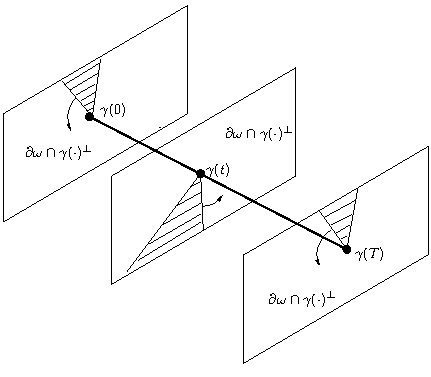
\includegraphics[width=7.2cm]{fig1-complete.pdf}
\end{center}
\caption{Locally around $\gamma(t)$, $\partial\omega\cap\gamma(t)^\perp$ is the complement of the hatched area.}\label{fig1}
\end{figure}

Now, we assume that, as $t>0$ increases, these sections rotate with such a speed that, along $[0,T]$, the entire vertical hyperplane is scanned by the section with $\omega$. If the speed of rotation is exactly $T/2\pi$ then it can be proved that $\ell^T(\mathring{\omega})=0$ and $\ell^T(\overline\omega)=1-2\varepsilon$.

This example shows that Assumption \eqref{thm_geomii}, or its generalization given in Remark~\ref{remgen}, cannot be weakened too much.
The idea here is to consider a subset $\omega$ such that the section of $\partial\omega$ with the vertical hyperplane $\gamma(\cdot)^\perp$ has locally the shape of the hypograph of an absolute value, which is rotating along $\gamma(\cdot)$.

Similar examples can as well be designed with checkerboard-shaped domains $\omega$, thus underlining that in \cite{Burq2017,BurqGerard2018} it was important to consider checkerboards in dimension~$2$.

\item Surprisingly, the result is wrong if the metric $g$ is not $C^2$. A counterexample is the following.

Let $M$ be a pill-shaped two-dimensional manifold given by the union of a cylinder of finite length, at the extremities of which we glue two hemispheres (domain also obtained by rotating a 2D stadium in $\R^3$ around its longest symmetry axis; or, take the unit sphere in $\R^3$, cut it at the equator, separate the two hemispheres and glue them with, in between, a cylinder of arbitrary length), and endow it with the induced Euclidean metric (see Figure \ref{fig2}).
\begin{figure}[htb]
\vspace*{-5pt}
\begin{center}
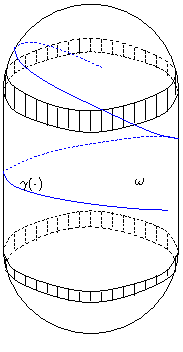
\includegraphics[width=3cm]{fig2-complete-v2.pdf}
\end{center}
\vspace*{-5pt}
\caption{$M$ is pill-shaped and $\omega$ is the complement of the hatched area.}\label{fig2}
\end{figure}

Then the metric is not $C^2$ at the gluing circles. Now, take $\omega$ defined as the union of the open cylinder with two open spherical caps (\ie the union of the two hemispheres of which we remove latitudes between $0$ and some $\varepsilon>0$). Then $\ell^T(\omega)=0$ for every $T>0$, because $\omega$ does not contain the rays consisting of the circles at the extremities of the cylinder. In contrast, $\ell^T(\overline\omega)$ may be arbitrarily close to $1$ as $T$ is large enough and $\varepsilon$ is small enough, and thus \eqref{mainineq} fails. This is because any ray of $M$ spending a~time $\pi$ in $M\setminus\omega$ spends then much time over the cylinder.

This shows that Assumption \eqref{thm_geomi} is sharp. In the above example, the metric is only $C^{1,1}$.

The example above is rather counter-intuitive. The assumption of a $C^2$ metric implies in some sense a global result on geodesic rays.
\end{itemize}

Our proof, given in Section \ref{sec_proof_thm_geom} hereafter, uses only elementary arguments of Riemannian geometry. It essentially relies on Lemma \ref{lemma2}, in which we establish that, given a grazing ray (\ie a ray propagating in $\partial\omega$), thanks to our assumption on $\omega$, we~can always construct neighbor rays, one of which being inside $\omega$ and the other being outside of $\omega$ for all times.

\subsection{Proof of Theorem \ref{thm_geom}}\label{sec_proof_thm_geom}
Without loss of generality, we take $\omega\subset M$ open.
We~will use several well known facts of Riemannian geometry, for which we refer to \cite{Berger}.

\begin{lemma}\label{lemma1}
There exists $\gamma\in\Gamma$ such that $\ell^T(\omega) = \frac{1}{T}\int_0^T\chi_\omega(\gamma(t))\, dt$, \ie the infimum in the definition \eqref{defg2} of $\ell^T(\omega)$ is reached.
\end{lemma}

\begin{proof}
Let $(\gamma_k)_{k\in\N}$ be a sequence of geodesic rays such that $\frac{1}{T}\int_0^T\chi_\omega(\gamma_k(t))\, dt \rightarrow \ell^T(\omega)$. By compactness of geodesics, {taking a subsequence if necessary,} $\gamma_k(\cdot)$ converges uniformly to some geodesic ray $\gamma(\cdot)$ on $[0,T]$.

Let $t\in[0,T]$ be arbitrary. If $\gamma(t)\in \omega$ then for $k$ large enough we have $\gamma_k(t)\in \omega$, and thus $1=\chi_{\omega}(\gamma(t))\leq \chi_{\omega}(\gamma_k(t))=1$. If $\gamma(t)\in M\setminus\omega$ then $0=\chi_{\omega}(\gamma(t))\leq \chi_{\omega}(\gamma_k(t))$ for any $k$. In all cases, we have obtained the inequality
\[
\chi_{\omega}(\gamma(t)) \leq \liminf_{k\rightarrow+\infty} \chi_{\omega}(\gamma_k(t))
\]
for every $t\in[0,T]$.
By the Fatou lemma, we infer that
\begin{multline*}
\ell^T(\omega)\leq \frac{1}{T}\int_0^T\chi_\omega(\gamma(t))\, dt \leq \frac{1}{T}\int_0^T \liminf_{k\rightarrow+\infty}\chi_\omega(\gamma_k(t))\, dt \\
\leq \liminf_{k\rightarrow+\infty} \frac{1}{T}\int_0^T \chi_\omega(\gamma_k(t))\, dt = \ell^T(\omega).
\end{multline*}
The lemma follows.
\end{proof}

If the ray $\gamma$ given by Lemma \ref{lemma1} is not grazing $\omega$, \ie if $\int_0^T\chi_{\partial\omega}(\gamma(t))\, dt=0$, then $\int_0^T\chi_{\omega}(\gamma(t))\, dt=\int_0^T\chi_{\overline\omega}(\gamma(t))\, dt$ and thus $\ell^T(\overline\omega)\leq \frac{1}{T} \int_0^T\chi_{\overline\omega}(\gamma(t))\, dt \leq \ell^T(\omega)$ and hence $\ell^T(\overline\omega)=\ell^T(\omega)$. So in this case there is nothing to prove.

In what follows we assume that the ray $\gamma$ given by Lemma \ref{lemma1} is grazing, \ie $\int_0^T\chi_{\partial\omega}(\gamma(t))\, dt>0$. Assume that $\gamma(t) = \pi\circ\varphi_t(x_0,\xi_0)$ with $x_0\in M$ and $\xi_0\in S_{x_0}^*M$. Here, $S_{x_0}^*M$ denotes the unit cotangent bundle at $x_0$ (\ie $\Vert\xi_0\Vert_{g^\star}=1$, where $g^*$ is the cometric), $(\varphi_t)_{t\in\R}$ is the geodesic flow on $S^*M$ and $\pi:S^*M\rightarrow M$ is the canonical projection.

\begin{lemma}\label{lemma2}
There exists a continuous path of points $s\mapsto x_s\in M$, passing through~$x_0$ at $s=0$, such that, setting $\gamma_s(t) = \pi\circ\varphi_t(x_s,\xi_0)$, we have
\begin{equation} \label{transverse}
\lim_{s\rightarrow 0} \left( \chi_{\overline\omega}(\gamma_s(t)) + \chi_{\overline\omega}(\gamma_{-s}(t)) \right) = 1
\end{equation}
for almost every $t\in[0,T]$ such that $\gamma(t)\in\partial\omega$.
\end{lemma}

\begin{proof}
To prove this fact, we assume that, in a local chart, $\gamma(t) = (t,0,\ldots,0)$. This is true at least in a neighborhood of $x_0=\gamma(0)=0$, and this holds true along $\gamma(\cdot)$ as long as there is no conjugate point. We also assume that, in this chart, any other geodesic ray starting at $(0,x_2^0,\ldots,x_n^0)$ in a neighborhood of $\gamma(0)=(0,\ldots,0)$, with codirection $\xi_0$, is given by $(t,x_2^0,\ldots,x_d^0)$ (projection onto $M$ of the extremal field). Here, we have set $d=\dim M$.
This classical construction of the so-called \emph{extremal field} can actually be done on any subinterval of $[0,T]$ along which there is no conjugate point.
Note that the set of conjugate times along $[0,T]$ is of Lebesgue measure zero.\footnote{This is a general fact in Riemannian geometry. Indeed, a conjugate time is a time at which a non-zero Jacobi field vanishes. Since Jacobi fields are solutions of a second-order ordinary differential equation, such times must be isolated, for otherwise the Jacobi field would vanish at the second order and thus would be identically zero.}
Let us search an appropriate $(d-1)$-tuple $(x_2^0,\ldots,x_d^0)\in\R^{d-1}\setminus\{0\}$ such that the family of points $x_s=(0,sx_2^0,\ldots,sx_d^0)$, $s\in(-1,1)$, gives \eqref{transverse}. Note that the geodesic ray starting at {$(x_s,\xi_0)$} is $\gamma_s(t) = (t,sx_2^0,\ldots,sx_d^0)$ in the local chart.

In what follows, we set $N=\partial\omega= \overline\omega \setminus \mathring{\omega} = \overline\omega \setminus \omega$ ($\omega$ is open).
By assumption, $\omega$~is an embedded $C^1$ submanifold of $M$ with boundary and one has $\dim N=d-1$. By~assumption, in a neighborhood $U$ of any point of $N$, the set $N\cap U$ is a codimension-one hypersurface of $M$, written as $F=0$ with $F:U\rightarrow\R$ of class $C^1$, which is separating $\omega$ and $M\setminus\omega$ in the sense that $\omega\cap U=\{F<0\}$, $N=\{F=0\}$ and $M\setminus\omega=\{F\geq 0\}$.

It suffices to prove that, for almost every time $t$ at which $\gamma_0(t)=\gamma(t)\in N$ and $\dot\gamma(t)\in T_{\gamma(t)}N$, the points $\gamma_s(t)$ and $\gamma_{-s}(t)$ are on different sides with respect to the (locally) separating manifold $N$ for $s$ small enough.

This is obvious when $\gamma$ is transverse to $N$.
We set
\[
\Omega=\{t\in[0,T] \mid \gamma(t)\in N,\, \dot\gamma(t)\in T_{\gamma(t)}N \}.
\]
It is a closed subset of $[0,T]$.
Let $t\in\Omega$. In the local chart the tangent space $T_{\gamma(t)}N$ is an hyperplane of $\R^n$ containing the line $\R(1,0,\ldots,0)$. Its projection onto $\{0\}\times\R^{d-1}$ (the hyperplane orthogonal to the line $\gamma(\cdot)$) is an hyperplane of $\{0\}\times\R^{d-1}$, of normal vector $(0,v(t))$ with $v(t)\in\R^{d-1}$ of Euclidean norm $1$. Since only the direction of $v(t)$ is important, we assume that $v(t)\in \mathbb{P}^{d-2}(\R)$, the projective space.

We claim that:
\begin{quote}
\textit{There exists $V\in \mathbb{P}^{d-2}(\R)$ such that $\langle V,v(t)\rangle\neq 0$ for almost every $t\in\Omega$}.
\end{quote}
With this result, setting $V=(x_2^0,\ldots,x_d^0)$, the points $x_s$ defined above give the lemma.

Let us now prove the claim.
We define $A=\{ (t,V)\in\Omega\times\mathbb{P}^{d-2}(\R)\mid \langle V,v(t)\rangle=0\}$. By definition, given $(t,V)\in\Omega\times\mathbb{P}^{d-2}(\R)$ we have $\chi_A(t,V)=1$ when $V\in v(t)^\perp$. Since $v(t)^\perp\cap\mathbb{P}^{d-2}(\R)$ is of codimension one in $\mathbb{P}^{d-2}(\R)$, we have $\int_{\mathbb{P}^{d-2}(\R)} \chi_A(t,V)\, d\mathcal{H}^{d-2}=0$ for every $t\in\Omega$, where we have endowed $\mathbb{P}^{d-2}(\R)$ with the Hausdorff measure $\mathcal{H}^{n-2}$. Therefore, by the Fubini theorem,
\[
0 = \int_\Omega \int_{\mathbb{P}^{d-2}(\R)} \chi_A(t,V)\, d\mathcal{H}^{d-2}\, dt = \int_{\mathbb{P}^{d-2}(\R)} \int_\Omega \chi_A(t,V)\, dt\, d\mathcal{H}^{d-2}
\]
and thus $\int_\Omega \chi_A(t,V)\, dt=0$ for almost every $V\in\mathbb{P}^{d-2}(\R)$. Fixing such a $V$, it follows that $\chi_A(t,V)=0$ for almost every $t\in\Omega$, and the claim is proved.
\end{proof}

In view of proving Remark \ref{remgen}, note that the argument above still works in dimension~$2$ with $\omega$ piecewise $C^1$ (but not in dimension greater than or equal to $3$: see the counterexample given in Section \ref{sec1}).
In more general, in any dimension, the argument above still works if $\omega$ is such that, for almost every time $t$, the subdifferential at $\gamma(t)$ of $\partial\omega\cap\gamma(\cdot)^\perp$ is a singleton.

At this step, we have embedded the ray $\gamma$ given by Lemma \ref{lemma1} into a family of rays~$\gamma_s$ which enjoy a kind of transversality property with respect to $N=\partial\omega$.
Let us consider the partition\vspace*{-3pt}
\[
[0,T] = A_1\cup A_2\cup A_3
\]
into three disjoint measurable sets, with
\begin{equation*}
\begin{split}
A_1 &= \{ t\in[0,T]\mid \gamma(t)\in\omega \},\\
A_2 &= \{ t\in[0,T]\mid \gamma(t)\in M\setminus\overline\omega \},\\
A_3 &= \{ t\in[0,T]\mid \gamma(t)\in\partial\omega \}.
\end{split}
\end{equation*}
Since $\gamma_s(\cdot)$ converges uniformly to $\gamma(\cdot)$ as $s\rightarrow 0$ and since $\omega$ and $M\setminus\overline\omega$ are open, we~have:\vspace*{-3pt}
\begin{align*}
\lim_{s\rightarrow 0} \left( \chi_{\overline\omega}(\gamma_s(t)) + \chi_{\overline\omega}(\gamma_{-s}(t)) \right) &= 2\quad\text{for every $t\in A_1$;}\\
\lim_{s\rightarrow 0} \left( \chi_{\overline\omega}(\gamma_s(t)) + \chi_{\overline\omega}(\gamma_{-s}(t)) \right) &= 0\quad\text{for every $t\in A_2$;}\\
\lim_{s\rightarrow 0} \left( \chi_{\overline\omega}(\gamma_s(t)) + \chi_{\overline\omega}(\gamma_{-s}(t)) \right) &= 1\quad\text{for almost every $t\in A_3$ (by Lemma \ref{lemma2}).}
\end{align*}
By the Lebesgue dominated convergence theorem, we infer that\vspace*{-3pt}
\[
\lim_{s\rightarrow 0} \int_0^T \left( \chi_{\overline\omega}(\gamma_s(t)) + \chi_{\overline\omega}(\gamma_{-s}(t)) \right) dt = 2\vert A_1\vert + \vert A_3\vert.
\]
Now, on the one part, by the first step we have $\frac{1}{T} \vert A_1\vert = \frac{1}{T} \int_0^T \chi_{\omega}(\gamma(t)) = \ell^T(\omega)$.
On~the other part, since $A_1$ and $A_3$ are disjoint we have $\frac{1}{T} ( \vert A_1\vert + \vert A_3\vert ) \leq 1$. Hence\vspace*{-3pt}
\[
\lim_{s\rightarrow 0} \frac{1}{T} \int_0^T \left( \chi_{\overline\omega}(\gamma_s(t)) + \chi_{\overline\omega}(\gamma_{-s}(t)) \right) dt \leq \ell^T(\omega)+1.
\]
Since $\ell^T(\overline\omega)\leq \frac{1}{T} \int_0^T \chi_{\overline\omega}(\gamma_{\pm s}(t)) dt$ for every $s$ by definition, we infer that $2 \ell^T(\overline\omega) \leq \ell^T(\omega)+1$. Theorem \ref{thm_geom} is proved.

\section{Proof of Theorem \ref{thm_random}}\label{sec_random}
Theorem \ref{thm_random} states that, given any $T>0$ and any $ \varepsilon \in [0, 1]$, the random variable $\ell^T(\omega_\varepsilon^n)$ converges in probability to $\varepsilon$ as $n\to +\infty$, \ie
\[
\lim_{n\to +\infty}\mathbb{P}\left(\vert\ell^T(\omega_\varepsilon^n) - \varepsilon \vert \geq \delta\right) = 0 \qquad \forall \delta>0.
\]
This section is organized as follows.
We make a preliminary remark in Section \ref{sec_prelim}.
In Section \ref{sec:sketch}, we give the successive steps of the proof, involving intermediate lemmas that are proved. One of the main ingredients of the proof of Theorem \ref{thm_random} is a large deviation property which is established in Section \ref{sec:LD}.
In Section \ref{sec_proof_cor_optimforme}, we also provide a proof of Corollary \ref{cor_optimforme}.

\subsection{Preliminaries}\label{sec_prelim}
For any geodesic ray $\gamma\!\in\!\Gamma$ and any measurable subset $\omega\!\subset\!M$, we set\vspace*{-3pt}
\begin{equation*}
m^T_\gamma(\omega) = \frac{1}{T}\int_0^T\chi_\omega(\gamma(t))\, dt,
\end{equation*}
so that\vspace*{-3pt}
\begin{equation}\label{lTmT}
\ell^T(\omega) = \inf_{\gamma \in \Gamma} m^T_\gamma(\omega).
\end{equation}

\begin{lemma}\label{lem3hv}
Given any measurable {closed} subset $\omega\subset M$, the mapping $\Gamma\ni \gamma \mapsto m^T_\gamma(\omega)$ is upper semi-continuous.

Given any $\omega$ that is a union of {closed} squares from the grid $\mathcal{G}^n$ with $n$ fixed, the mapping $\Gamma\ni \gamma \mapsto m^T_\gamma(\omega)$ is continuous at every $\gamma\in\Gamma$ that is neither horizontal nor vertical, or, that is horizontal {or} vertical but meets no corner (by definition, a corner is a point $(i/n,j/n)$ in $[0,1]^2$, for some $(i,j)\in\{0,\ldots,n\}^2$).
\end{lemma}

\begin{proof}
{Let $\gamma\in\Gamma$ and let $(\gamma_k)_{k\in\N}$ be a sequence of $\Gamma$ converging to $\gamma$. Let us prove that
\begin{equation}\label{13:32}
m_\gamma^T(\omega) \geq \limsup_{k\rightarrow+\infty} m_{\gamma_k}^T(\omega).
\end{equation}
Let $t\in[0,T]$. If $\gamma(t)\in\omega$ then $\chi_\omega(\gamma(t)) \geq \chi_\omega(\gamma_k(t))$ for every $k$. If $\gamma(t)\in M\setminus\omega$ then, since $M\setminus\omega$ is open, $\gamma_k(t)\in M\setminus\omega$ for $k$ large enough and thus $\chi_\omega(\gamma(t)) = \chi_\omega(\gamma_k(t)) = 0$. Now \eqref{13:32} follows.
}

Let us prove the second part of the lemma.
Let $\gamma\in\Gamma$ that is neither horizontal nor vertical, or, that is horizontal or vertical but meets no corner. Let $(\gamma_k)_{k\in \N}$ be a sequence of geodesic rays converging to $\gamma\in \Gamma$.
Writing
\[
\chi_{\omega}=\sum_{i,j=1}^n\tau(i,j)\chi_{c_{ij}^n},
\]
where $\tau(i,j)=1$ if $c_{ij}^n\subset \omega$ and $\tau(i,j)=0$ otherwise, and noting that
\[
m^T_{\gamma_k}(\omega)=\sum_{i,j=1}^n\tau(i,j)m^T_{\gamma_k}(c_{ij}^n),
\]
we have to prove that $m^T_{\gamma_k}(c_{ij}^n)$ converges to $m^T_{\gamma}(c_{ij}^n)$ as $k\rightarrow+\infty$. This follows from the dominated convergence theorem and from the fact that $(\chi_{c_{ij}^n}(\gamma_k) )_{k\in \N}$ converges almost everywhere to $\chi_{c_{ij}^n}(\gamma) $. The latter claim can be shown by distinguishing between two cases: if $\gamma(t)\in \mathring{c}_{ij}^n$ then for $k$ large enough we have $\gamma_k(t)\in \mathring{c}_{ij}^n$ and $\chi_{c_{ij}^n}(\gamma_k(t))=\chi_{c_{ij}^n}(\gamma(t))=1$. The same conclusion remains true if $\gamma(t)\notin c_{ij}^n$. Since the set of $t$ such that $\gamma(t)\in \partial c_{ij}^n$ is finite {(this follows from the assumptions on $\gamma$)},
the lemma follows.
\end{proof}

{
Note that $\gamma\mapsto m_\gamma^T$ may fail to be continuous at some $\gamma\in\Gamma$ that is horizontal or vertical and meets a corner. For such geodesic rays $\gamma$, we will see that it is relevant to define the following quantity. Given any $\gamma\in\Gamma$, we set $\widetilde m^T_\gamma(\omega) = m^T_\gamma(\omega)$ if $\gamma$ is neither horizontal nor vertical, or is horizontal or vertical but meets no corner. When $\gamma$ is horizontal or vertical and meets a corner, we set
\begin{equation}\label{def_tildemT}
\widetilde m^T_\gamma(\omega) = \inf_{(\gamma_k')_{k\in \N}}\liminf_{k\to +\infty} m^T_{\gamma'_k}(\omega),
\end{equation}
where the infimum is taken over the set of sequences of geodesic rays $(\gamma'_k)_{k\in\N}$ converging to $\gamma$ such that, for every $k\in\N$, $\gamma'_k([0,T])$ is obtained by rotating $\gamma([0,T])$ around a corner of the grid through which $\gamma$ passes.
Of course, we have $\ell^T(\omega) \leq \widetilde m^T_\gamma(\omega) \leq m^T_\gamma(\omega)$ and thus
\begin{equation*}
\ell^T(\omega) = \inf_{\gamma \in \Gamma} \widetilde m^T_\gamma(\omega).
\end{equation*}
Note that $\gamma\mapsto \widetilde m^T_\gamma(\omega)$ may also fail to be continuous.
We will see that this quantity $\widetilde m^T_\gamma(\omega)$ is important to obtain the inequality \eqref{semicont} in the proof of Lemma~\ref{lem:compare}, item \eqref{lem:compareg3g4}, and in order to treat the case of horizontal or vertical rays in the proof of Lemma \ref{lem:limprobg4}.
}

\subsection{Proof of Theorem \ref{thm_random}}\label{sec:sketch}
For every $(i,j)\in \{1,\ldots,n\}^2$, let $X_{ij}^n$ be the random variable equal to $1$ whenever $c_{ij}^n\subset\omega_\varepsilon^n$ and $0$ otherwise.
Recall that, assuming that all square cells of the grid are initially white, when ranging over the grid, for each cell we randomly darken the cell with a probability $\varepsilon$ (Bernoulli law) and in this case we set $X_{ij}^n=1$; otherwise we let $X_{ij}^n=0$.
By construction, the random laws $(X_{ij}^n)_{1\leq i,j\leq n}$ are independent and identically distributed (i.i.d.), of expectation $\varepsilon$ and of variance $\varepsilon(1-\varepsilon)$.

Given any fixed geodesic ray $\gamma\in\Gamma$, we denote by $t_{ij}^n(\gamma)$ the time spent by $\gamma$ in the square cell $c_{ij}^n$. We have $\sum_{i,j=1}^nt_{ij}^n(\gamma)=T$.
It may happen that $\gamma$ crosses several times (at most $T+1$ times) the square cell $c_{ij}^n$, and in this case $t_{ij}^n(\gamma)$ is the sum of several passage times; since the maximal time spent in $c_{ij}^n$ by a ray in one passage is $\sfrac{\sqrt{2}}{n}$, we have $t_{ij}^n(\gamma) \leq (T+1) \sfrac{\sqrt{2}}{n}$.
Summing up, we have
\begin{equation}\label{propriete_tij}
\forall (i,j)\in \{1,\ldots,n\}^2\qquad \frac{t_{ij}^n(\gamma)}{T} \leq \frac{T+1}{T}\, \frac{\sqrt{2}}{n}
\qquad\textrm{and}\qquad
\sum_{i,j=1}^n \frac{t_{ij}^n(\gamma)}{T} = 1
\end{equation}
and we also note that
\begin{equation}\label{18:26}
m^T_\gamma(\omega_\varepsilon^n) = \frac{1}{T} \int_0^{T} \chi_{\omega_\varepsilon^n} (\gamma(t) ) \, dt = \sum_{i,j=1}^n \frac{t_{ij}^n(\gamma)}{T}\, X_{ij}^n.
\end{equation}
In particular, the random variable $m^T_\gamma(\omega_\varepsilon^n)$ is a weighted sum of independent Bernoulli laws, and thus its expectation is
\begin{equation}\label{expectation_m}
\mathbb{E}\,m^T_\gamma(\omega_\varepsilon^n) = \varepsilon
\end{equation}
and its variance is
\begin{equation}\label{variance_m}
\mathrm{Var}\,m^T_\gamma(\omega_\varepsilon^n) = \sum_{i,j=1}^n \Bigl( \frac{t_{ij}^n(\gamma)}{T} \Bigr)^2 \varepsilon(1-\varepsilon)
\leq \frac{T+1}{T}\, \frac{\sqrt{2}}{n}\,\varepsilon(1-\varepsilon),
\end{equation}
where we have used \eqref{propriete_tij} and the fact that $0\leq \sfrac{t_{ij}^n(\gamma)}{T}\leq 1$.

To prove Theorem \ref{thm_random}, we have to prove that, given any $T>0$ and any $\varepsilon\in[0,1]$, for every $\delta>0$ we have
\begin{enumeratei}
\item\label{igd1} $\displaystyle\lim_{n\to +\infty} \mathbb{P}\left( \ell^T(\omega_\varepsilon^n) \leq \varepsilon + \delta \right) = 1$,
\item\label{igd2} $\displaystyle\lim_{n\to +\infty} \mathbb{P}\left( \ell^T(\omega_\varepsilon^n) \geq \varepsilon - \delta \right) = 1$, or equivalently, $\displaystyle\lim_{n\to +\infty} \mathbb{P}\left( \ell^T(\omega_\varepsilon^n) \leq \varepsilon - \delta \right) = 0$.
\end{enumeratei}

\subsubsection*{Proof of \eqref{igd1}}
Using \eqref{lTmT} and \eqref{18:26}, we have
\begin{equation}\label{17:59}
\ell^T(\omega_\varepsilon^n) \leq m^T_\gamma(\omega_\varepsilon^n).
\end{equation}
Applying the Bienaymé-Tchebychev inequality to the random variable $m^T_\gamma(\omega_\varepsilon^n)$, we~have
\[
\mathbb{P}\left( \vert m^T_\gamma(\omega_\varepsilon^n)-\varepsilon \vert\geq \delta \right) \leq \frac{T+1}{T}\, \frac{\sqrt{2}}{n}\,\frac{\varepsilon(1-\varepsilon)}{\delta^2} \qquad\forall\gamma\in\Gamma
\]
and thus, using \eqref{expectation_m} and \eqref{variance_m},
\begin{equation}\label{11:37}
\lim_{n\to +\infty} \mathbb{P}\left( m^T_\gamma(\omega_\varepsilon^n) \leq \varepsilon + \delta\right) = 1.
\end{equation}
Finally, \eqref{igd1} follows from \eqref{17:59} and \eqref{11:37}.

\subsubsection*{Proof of \eqref{igd2}.} Establishing \eqref{igd2} is much more difficult. We proceed in several steps, by proving the following successive lemmas that are in order.

\begin{lemma} \label{lem:smallT}
If \eqref{igd2} is true for every $T \in (0,1)$, then it is true for every $T>0$.
\end{lemma}

Thanks to Lemma \ref{lem:smallT} (proved below), we now assume that $0<T<1$.
{This has the following pleasant consequence: any geodesic ray $\gamma\in\Gamma$ crosses a given cell $c_{ij}$ at most one time over $[0,T]$, \ie $\{ t\in[0,T]\mid \gamma(t)\in c_{ij}\}$ is connected. This will make easier the computation of crossing times, in the proofs of the forthcoming lemmas.}

Let us introduce some notations. Let $\Gamma^0$, $\Gamma^1$ and $\Gamma^2$ be the sets of geodesic rays of $M=\mathbb{T}^2$ meeting respectively zero, at least one and at least two corners of the grid $\mathcal{G}^n$ (by definition, a corner is a point $(i/n,j/n)$ in $[0,1]^2$, for some $(i,j)\in\{0,\ldots,n\}^2$).
{Note that $\Gamma^2\subset \Gamma^1$.}

Given any $\omega\subset M$ that is the union of disjoint closed square cells of $\mathcal{G}^n$, we have
\[
\ell^T(\omega) = \inf_{\gamma\in \Gamma^0 \cup \Gamma^1} m^T_\gamma(\omega).
\]
We also define
\[
\ell_{\Gamma^1}^T(\omega) = \inf_{\gamma\in \Gamma^1} m^T_\gamma(\omega),\qquad
\ell_{\Gamma^2}^T(\omega) = \inf_{\gamma\in \Gamma^2} m^T_\gamma(\omega).
\]
Of course, we have
\[
\ell^T(\omega) \leq \ell_{\Gamma^1}^T(\omega) \leq \ell_{\Gamma^2}^T(\omega).
\]

\begin{lemma}\label{lem:compare}
There exists $C>0$ such that, for every $n\in\N^*$, for every subset $\omega$ of $[0,1]^2$ that is a union of square cells of the grid $\mathcal{G}_n$, we have:
\begin{enumeratea}
\item\label{lem:compareg2g3}
$\ell_{\Gamma^1}^T(\omega)\leq \ell^T(\omega) +\sfrac{C}{n}$;
\item\label{lem:compareg3g4}
$\ell_{\Gamma^2}^T(\omega)\leq \ell_{\Gamma^1}^T(\omega)+\sfrac{C}{n}$.
\end{enumeratea}
\end{lemma}

\begin{lemma}\label{lem:limprobg4}
We have $\displaystyle \lim_{n\to +\infty}\mathbb{P}\left(\ell_{\Gamma^2}^T(\omega_\varepsilon^n)\leq \varepsilon-\delta\right)=0$.
\end{lemma}

Finally, \eqref{igd2} follows from the above lemmas, that are proved hereafter.

\subsubsection{Proof of Lemma \ref{lem:smallT}}
Let $T\!\geq\!1$ and let $m\!\in\!\N^*$ be such that \hbox{$T'\!=\!\sfrac{T}{m}\!\in\!(0,1)$}.
Let us prove that
\begin{equation}\label{eq:metz1225}
\ell^T(\omega_\varepsilon^n) \geq \ell^{T'}(\omega_\varepsilon^n).
\end{equation}
Given any $\rho>0$, let $\gamma$ be a geodesic ray such that
\[
\ell^T(\omega_\varepsilon^n) + \rho \geq \frac{1}{T} \int_0^{T} \chi_{\omega_\varepsilon^n} (\gamma(t) ) \, dt.
\]
Setting $\gamma_k(\cdot)=\gamma(k T'+ \cdot)$ for every $k \in \{ 0, \ldots, m-1\}$, we have
\begin{multline*}
\ell^T(\omega_\varepsilon^n) + \rho \geq \frac{1}{T} \int_0^{T} \chi_{\omega_\varepsilon^n} (\gamma(t) ) \, dt = \frac{1}{T} \sum_{k=0}^{m-1} \int_0^{T'} \chi_{\omega_\varepsilon^n} (\gamma_k(t) ) \, dt\\[-5pt]
\geq \frac{1}{T} \sum_{k=0}^{m-1} T' \ell^{T'}(\omega_\varepsilon^n) = \ell^{T'}(\omega_\varepsilon^n).
\end{multline*}
Letting $\rho$ tend to 0, we obtain \eqref{eq:metz1225}.

Since $0<T'<1$, \eqref{igd2} is true for this final time $T'$, \ie
\[
\displaystyle\lim_{n\to +\infty} \mathbb{P}\left( \ell^{T'}(\omega_\varepsilon^n) \geq \varepsilon - \delta \right) = 1.
\]
Therefore, using \eqref{eq:metz1225}, we obtain \eqref{igd2} for the final time $T$.

\Subsubsection{Proof of Lemma \ref{lem:compare}}

\subsubsection*{Proof of item \eqref{lem:compareg2g3}.}
Let $\gamma\in\Gamma$ be such that
\begin{equation} \label{smallm}
\ell^T(\omega)\leq m^T_\gamma(\omega) < \ell^T(\omega) + \frac{1}{nT}.
\end{equation}
If $\gamma\in\Gamma^1$ then we are done. Hence, in what follows we assume that $\gamma\in\Gamma^0$, \ie that~$\gamma$ meets no corner of the grid.

Without loss of generality, we can assume that the ray $\gamma$ is neither horizontal nor vertical. Indeed, if $\gamma$ is horizontal or vertical, since $\gamma$ meets no corner, it follows from Lemma \ref{lem3hv} that $m^T_\gamma$ is continuous at $\gamma$. Hence, it is possible to rotate slightly $\gamma$ so that~$\gamma$ is neither horizontal nor vertical and still satisfies \eqref{smallm}.

Let $\boldsymbol{n}\in\R^2$ be a unit vector orthogonal to $\gamma'(0)$.
For every $s\in\R$, we denote by $\mathcal{T}_{s\boldsymbol{n}}$ the translation of vector $s\boldsymbol{n}$ and we define the translated geodesic ray $\gamma_s= \mathcal{T}_{s\boldsymbol{n}} \circ \gamma$ (which is neither horizontal nor vertical). By continuity, $\gamma_s$ meets the same square cells as $\gamma$ if $\vert s\vert$ is small enough. Let $I(\gamma)$ denote the subset of all pairs $(i,j)\in\{1,\ldots,n\}^2$ such that $\gamma$ crosses the cell squares $c_{ij}^n$. For $\vert s\vert$ small enough, we have
\[
m^T_{\gamma_s}(\omega)=\sum_{(i,j)\in I(\gamma)} \frac{t_{ij}^n(\gamma_s)}{T}\, X_{ij}^n,
\]
where $t_{ij}^n(\gamma_s)$ is the time spent by $\gamma_s$ in $c_{ij}^n$.
Denoting by $I'(\gamma)$ the set of $(i,j)\in I(\gamma)$ such that $\gamma(0), \gamma(T) \notin \mathring{c}_{ij}^n$ (note that $\# I(\gamma) - 2 \leq \# I '(\gamma) \leq \# I(\gamma)$ {and that these conditions do not depend on $s$ for $\vert s\vert$ small enough, hence $I '(\gamma_s)=I '(\gamma)$}), an easy geometric argument shows that, for $(i,j)\in I'(\gamma)$, the function $s\mapsto t_{ij}^n(\gamma_s)$ is affine and nonconstant with respect to $s$.
Hence,
\begin{equation}\label{defMom}
M_{\gamma_s}(\omega) = \sum_{(i,j) \in I'(\gamma)} \frac{t_{ij}^n(\gamma_s)}{T}\,X_{ij}^n
\end{equation}
is also an affine function of $s$.
Replacing $s$ by $-s$ if necessary, we infer the existence of a threshold $s_0 >0$ such that {$\gamma_s\in\Gamma^0$ for $s\in[0,s_0)$} and $\gamma_{s_0}\in\Gamma^1$, and the mapping $s\mapsto M_{\gamma_s}(\omega)$ is {continuous and nonincreasing} on $[0,s_0]$ {(continuity is because, for every~$s$, $\gamma_s$ is neither vertical nor horizontal since it is a translation of $\gamma$)}.
Since $\gamma_{s_0}\in\Gamma^1$, we have
\begin{equation}\label{11:19}
\ell_{\Gamma^1}^T(\omega) \leq m^T_{\gamma_{s_0}} (\omega).
\end{equation}
Besides, we have, {for every $s\in[0,s_0]$,}
\begin{equation}\label{MTforalls}
M_{\gamma_s}(\omega)\leq m^T_{\gamma_s}(\omega) \leq M_{\gamma_s}(\omega) + \sum_{(i,j) \in I(\gamma) \setminus I'(\gamma) } \frac{t_{ij}^n(\gamma_s)}{T}\, X_{ij}^n \leq M_{\gamma_s}(\omega) + \frac{2 \sqrt{2}}{nT}.
\end{equation}
Hence, in particular, {using that (by Lemma \ref{lem3hv}) $s\mapsto m^T_{\gamma_s} (\omega)$ is continuous because $\gamma_s$ is neither horizontal nor vertical,}
\begin{equation}\label{11:20}
m^T_{\gamma_{s_0}} (\omega) \leq M_{\gamma_{s_0}} (\omega) + \frac{2 \sqrt{2}}{nT}.
\end{equation}
Since the mapping $s\mapsto M_{\gamma_s}(\omega)$ is nonincreasing on $[0,s_0]$ and $\gamma_0=\gamma$, we have $M_{\gamma_{s_0}} (\omega) \leq M_{\gamma} (\omega)$ and thus, using \eqref{MTforalls},
\begin{equation}\label{11:21}
M_{\gamma_{s_0}} (\omega) \leq m^T_\gamma(\omega).
\end{equation}
We finally infer from \eqref{smallm}, \eqref{11:19}, \eqref{11:20} and \eqref{11:21} that
\[
\ell_{\Gamma^1}^T(\omega) < \ell^T(\omega)+\frac{2 \sqrt{2}+ 1}{nT}.
\]
The conclusion follows.

\subsubsection*{Proof of item \eqref{lem:compareg3g4}}
Let $\gamma\in\Gamma^1$ be such that
\begin{equation} \label{smallm1}
\ell^T_{\Gamma^1}(\omega)\leq m^T_\gamma(\omega) < \ell^T_{\Gamma^1}(\omega) + \frac{1}{n}.
\end{equation}
If $\gamma\in\Gamma^2$ then we are done. Hence, in what follows we assume that $\gamma \in \Gamma^1 \setminus \Gamma^2$. It~suffices to find $\gamma' \in \Gamma^2$ such that
\begin{equation} \label{g3g4}
m^T_{\gamma'} (\omega) \leq m^T_{\gamma}(\omega) + \frac{C}{n}
\end{equation}
for some $C >0$ not depending on $\gamma$ and $n$. Indeed, then, it follows from \eqref{smallm1} and \eqref{g3g4} that
\[
\ell^T_{\Gamma^2}(\omega)\leq m^T_{\gamma'} (\omega)\leq m^T_{\gamma}(\omega) + \frac{C}{n}< \ell^T_{\Gamma^1}(\omega) + \frac{C+1}{n}
\]
and the item is proved.

Let us establish \eqref{g3g4}.
By definition, the geodesic ray $\gamma$ meets exactly one corner of the grid, denoted by $O$.
Let $R_\theta$ be the rotation centered at $O$ with angle $\theta$ and let $\gamma_\theta=r_\theta \circ \gamma \in\Gamma$. Recall that $I'(\gamma)$ stands for the set of all pairs $(i,j)\in \{1,\ldots,n\}^2$ such that $\gamma_\theta$ crosses $c_{ij}^n$ and $\gamma(0), \gamma(T) \notin \mathring{c}_{ij}^n$: these conditions do not depend on $\theta \in J= (\theta_-, \theta_+)$, where $\theta_-<0$ and $\theta_+ >0$ are thresholds such that $\gamma_\theta \notin \Gamma^2$ for every $\theta \in J$ and $\gamma_{\theta_\pm} \in \Gamma^2$. We define the {continuous} function $f$ on $J$ by $f(\theta)=M_{\gamma_\theta} (\omega)$, defined as in \eqref{defMom} but where $\gamma_\theta$ is obtained by rotation of $\gamma$ and not by translation. We extend $f$ by continuity on $\bar{J}$. The inequality \eqref{MTforalls} is valid as well for every $\theta\in \bar J$.

Note, however, that the functions $\theta\mapsto m_{\gamma_\theta}^T(\omega)$ and $\theta\mapsto M_{\gamma_\theta}(\omega)$ may fail to be continuous at $\theta_\pm$ (\ie we may have $f(\theta_\pm)\neq M_{\gamma_\theta}(\omega_\pm)$) whenever $\gamma_{\theta_\pm}$ is horizontal or vertical and meets a corner.

We claim that
\begin{equation} \label{minf}
\min(f(\theta_-), f(\theta_+)) \leq \min_{\theta\in\bar J} f(\theta) +\frac{K}{n}
\end{equation}
for some $K>0$ not depending on $n$ nor on $\gamma$.
Admitting temporarily \eqref{minf}, without loss of generality we assume that $f(\theta_-) \leq f(\theta_+ )$.
Let us prove that
\begin{equation} \label{semicont}
\widetilde m^T_{\gamma_{\theta_-}}(\omega) \leq f(\theta_-) + \frac{2 \sqrt{2}}{nT},
\end{equation}
where $\widetilde m^T_{\gamma}(\omega)$ is defined by \eqref{def_tildemT} in Section \ref{sec_prelim}.
When $\gamma_{\theta_-}$ is neither horizontal nor vertical, or is horizontal or vertical but meets no corner, we have $\widetilde m^T_{\gamma_{\theta_-}}(\omega) = m^T_{\gamma_{\theta_-}}(\omega)$ and \eqref{semicont} follows from \eqref{MTforalls} and from the fact that $f(\theta_-) = M_{\gamma_\theta}(\omega_-)$ (actually, \eqref{semicont} is an equality in this case).
When $\gamma_{\theta_-}$ is horizontal or vertical and meets a corner, it is the limit of $\gamma'_k = \gamma_{\theta_- + \frac{1}{k}}$ and then, by definition, $\widetilde m^T_{\gamma_{\theta_-}}(\omega) \leq m_{\gamma'_k}^T(\omega)$; but, using \eqref{MTforalls}, we have
\[
m_{\gamma'_k}^T(\omega) \leq M_{\gamma'_k}(\omega)+\frac{2\sqrt{2}}{nT} = f(\theta_-+\sfrac{1}{k})+\frac{2\sqrt{2}}{nT},
\]
whence \eqref{semicont} by continuity of $f$.

We infer from \eqref{minf} and \eqref{semicont} that
\[
\widetilde m^T_{\gamma_{\theta_-}}(\omega) \leq \min_{\theta\in\bar J} f(\theta) +\frac{K}{n} + \frac{2 \sqrt{2}}{nT}.
\]
Since $\min_{\theta\in\bar J} f(\theta) \leq f(0) = M_{\gamma}(\omega) \leq m^T_\gamma(\omega)$, we obtain
$\widetilde m^T_{\gamma_{\theta_-}}(\omega) \leq m^T_\gamma(\omega) +\sfrac{K'}{n}$
with $K'= K +\sfrac{2 \sqrt{2}}{T}$. By definition of $\widetilde m^T_{\gamma_{\theta_-}}(\omega)$ in \eqref{def_tildemT}, there exists a geodesic ray $\gamma'$ such that $\widetilde m^T_{\gamma_{\theta_-}}(\omega)+1/n \geq m^T_{\gamma'}(\omega)$.
Therefore, \eqref{g3g4} is proved by setting $C=K'+1$.

It remains to prove \eqref{minf}.
Let us first compute $f$ by deriving an explicit expression of $t_{ij}^n(\gamma_\theta)$. We claim that, for $(i,j)\in I(\gamma)$, there exists $(a_{ij},b_{ij})\in \{-n,\ldots,n\}^2$ such that
\begin{equation}\label{dim:metz1220}
t_{ij}^n(\gamma_\theta)=\frac{a_{ij}}{n\sin(\theta_0+\theta)}+\frac{b_{ij}}{n\cos(\theta_0+\theta)},
\end{equation}
where $\theta_0$ is the angle between the horizontal axis and the geodesic ray $\gamma$. Without loss of generality we assume that $\theta_0 \in [0,\pi/2]$. Note that $\theta_0 \in (0, \pi/2)$, because otherwise the two conditions $\gamma \in \Gamma_1$ and $\theta_0 \in \{0, \pi/2\}$ (\ie $\gamma$ is horizontal or vertical) would imply that $\gamma \in \Gamma_2$, which is not true.
This also implies that $J \subset (0, \pi/2)$.
\begin{figure}[htb]
\begin{center}
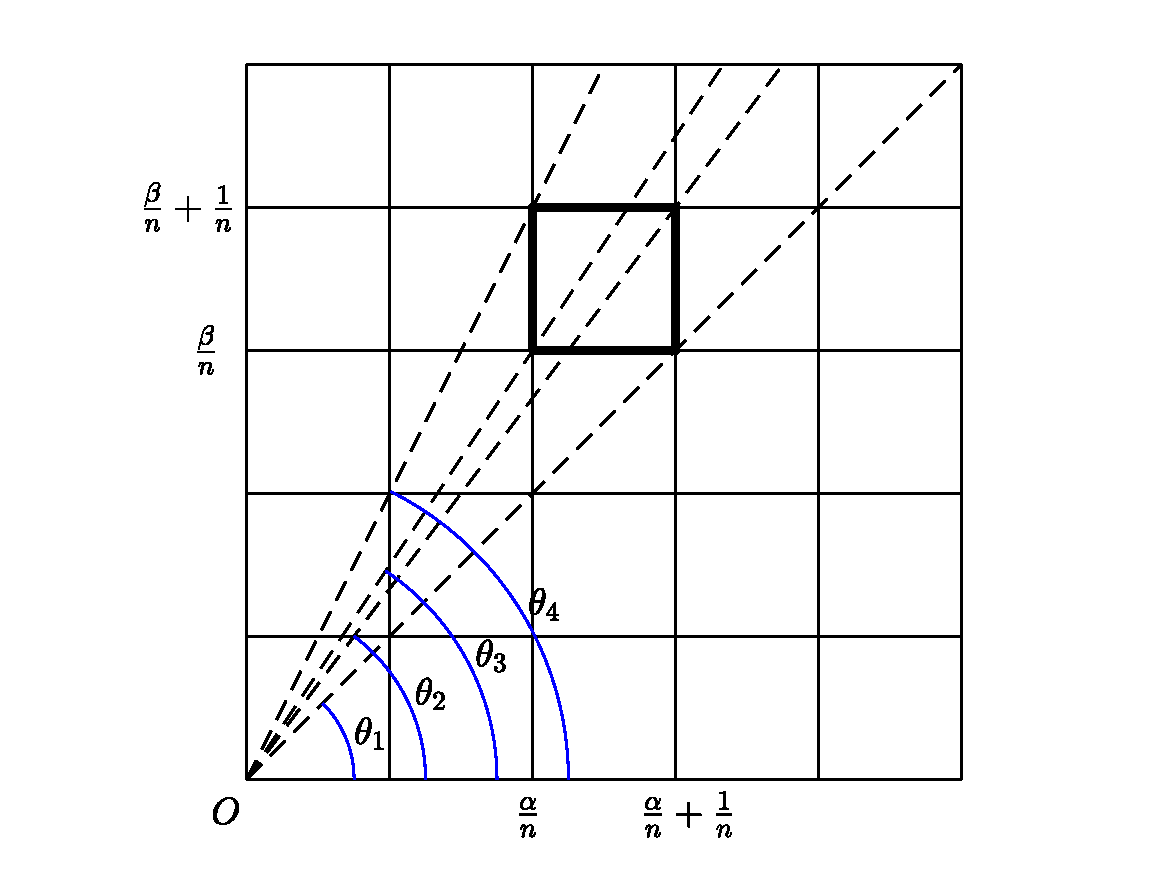
\includegraphics[width=9cm]{dessinQuad.pdf}
\caption{Particular geodesics issued from $O$ and meeting the square with bold boundary.}\label{figdessinQuad}
\end{center}
\end{figure}

Using the notations of Figure \ref{figdessinQuad} where the corner $O$ is assimilated to the origin, and focusing on the square $c_{ij}^n$ of vertices
\[
(\alpha/n,\beta/n),\ (\alpha/n+1/n,\beta/n),\ (\alpha/n+1/n,\beta/n+1/n)\text{ and }(\alpha/n,\beta/n+1/n),
\]
an elementary geometric reasoning gives
\[
t_{ij}^n(\gamma_\theta)=
\begin{cases}
\dfrac{\alpha+1}{n\cos{(\theta_0+\theta)}}-\dfrac{\beta}{n\sin{(\theta_0+\theta)}} & \text{if }\theta_0 + \theta\in [\theta_{1},\theta_2],\\[10pt]
\dfrac{1}{n\sin{(\theta_0+\theta)}} & \text{if }\theta_0 + \theta \in [\theta_2,\theta_3],\\[10pt]
\dfrac{\beta+1}{n\sin{(\theta_0+\theta)}}-\dfrac{\alpha}{n\cos{(\theta_0+\theta)}} & \text{if } \theta_0 +\theta\in [\theta_{3},\theta_{4}],
\end{cases}
\]
where $0<\theta_{1}<\theta_2<\theta_3<\theta_{4}<\pi/2$ are the angles between the horizontal axis and the particular geodesics passing through the corners of $c_{ij}^n$ (see Figure \ref{figdessinQuad}). Note that this formula is still satisfied when $\theta_1=0$ or $\theta_4=\pi/2$. In such cases, either $\alpha$ or $\beta$ vanishes.
The claim \eqref{dim:metz1220} is then proved.

Note that the rotation $R_\theta$ can be applied to $\gamma$ until the geodesic ray $\gamma_\theta$ meets a new corner. It is then easy to see that
\begin{equation} \label{thetapm}
-\theta_- \leq \frac{C}{n}, \qquad\theta_+ \leq \frac{C}{n},
\end{equation}
for some $C>0$ neither depending on $n$ nor on $\gamma$.

According to \eqref{dim:metz1220}, we have
\begin{equation}\label{metz:2248}
M_{\gamma_\theta }(\omega)=\frac{X_1}{\sin (\theta_0+\theta)}+\frac{X_2}{\cos (\theta_0+\theta)},
\end{equation}
with
\[
X_1=\frac{1}{n}\sum_{(i,j)\in I'(\gamma)}a_{ij} M_{\gamma_\theta}(c_{ij}^n)\quad \text{and}\quad X_2=\frac{1}{n}\sum_{(i,j)\in I'(\gamma)}b_{ij} M_{\gamma_\theta}(c_{ij}^n),
\]
for $\theta\in J$.
Moreover, we have
{
\[
\max (|X_1|,|X_2|)\leq \frac{1}{n}\,\# I'(\gamma)n\,\frac{\sqrt{2}}{nT}\leq 3
\]
because $\max (|a_{ij}|,|b_{ij}|) \leq n$, $M_{\gamma_\theta}(c_{ij}^n)\leq \sfrac{\sqrt{2}}{nT}$ and $\# I'(\gamma)\leq 2n$, the latter inequality following from the obvious observation that, when $\gamma$ leaves a square $c_{ij}^n$, then the next square that $\gamma$ enters must be of the form $c_{i'j'}$ with $i'=i+1$ or $j'=j+1$.
}

We are now in a position to establish \eqref{minf}. It is obvious if $\min_J f$ is reached at ${\theta_-}$ or~$\theta_+$. Let us then assume that $f$ reaches its minimum {in $(\theta_-,\theta_+)$}; without loss of generality, we assume that the minimum is reached at $\theta=0$. In~particular, $\left.\frac{d}{d\theta}\right|_{\theta=0}M_{\gamma_\theta}(\omega)=0$
which, using \eqref{metz:2248}, yields
\[
\frac{\cos (\theta_0)}{\sin ^2(\theta_0)}\,X_1=\frac{\sin (\theta_0)}{\cos ^2(\theta_0)}\,X_2.
\]
From \eqref{metz:2248}, we also have $f(0)=\sfrac{X_1}{\sin \theta_0}+\sfrac{X_2}{\cos \theta_0}$ and thus
$X_1=f(0) \sin^3(\theta_0)$ and $X_2=f(0) \cos^3(\theta_0)$, so that
\[
f(\theta)= M_{\gamma_\theta}(\omega)= f(0) \Bigl( \frac{\sin^3(\theta_0)}{\sin(\theta_0+\theta)} + \frac{\cos^3(\theta_0)}{\cos(\theta_0+\theta)} \Bigr).
\]
Now,
\[
f(\theta)-f(0)=f(0) \Bigl(\sin^3\theta_0\Bigl(\frac{1}{\sin (\theta_0+\theta)}-\frac{1}{\sin \theta_0}\Bigr) +\cos^3\theta_0\Bigl(\frac{1}{\cos (\theta_0+\theta)}-\frac{1}{\cos \theta_0}\Bigr)\Bigr).
\]
This computation shows that $\theta_0 + \theta_+ \neq \pi/2$ {and} $\theta_0+\theta_-\neq 0$. Otherwise, since $\theta_0 \notin \{0, \pi/2\}$, $f$ would be not bounded on $J$ when $\theta$ tends to $\theta_0 + \theta_+$ or $\theta_0 + \theta_-$, which is not true by definition of $f$.
This implies that
\begin{equation} \label{estimangle}
\arcsin( \sfrac{1}{nT}) \leq \theta_0 + \theta_- < \theta_0 + \theta_+ \leq \frac{\pi}{2} -\arcsin( \sfrac{1}{nT}).
\end{equation}
Indeed, set $\gamma_- = \gamma_{\theta_0+\theta_-}$. We know that $\gamma_-([0,T])$ contains at least two corners and is not horizontal (since $\theta_0+\theta_->0$). This means that its second coordinate (in $\R^2$) increases at least of $1/n$ between $0$ and $T$ and hence $T \sin(\theta_0 + \theta_-) \geq 1/n$. A similar argument gives the right-hand inequality in \eqref{estimangle}.

From now on, we let $n$ tend to $+\infty$. In particular, $\theta_0$ depends on $n$.
Let us prove that
\begin{equation} \label{f(theta-)}
f(\theta_-)-\min_J f =f(\theta_-) - f(0) \leq \frac{C}{n}.
\end{equation}
A similar argument will show that $f(\theta_+)-\min_J f \leq \sfrac{C}{n}$.
These two estimates imply~\eqref{minf} and hence complete the proof of the item \ref{lem:compareg3g4}.
It thus remains to prove
\eqref{f(theta-)}.
By the mean value theorem, there exists $\tilde \theta \in (0,|\theta_-|)$ such that
\[\frac{1}{\sin (\theta_0 + \theta_-)} - \frac{1}{\sin \theta_0}=\frac{\cos (\theta_0-\tilde \theta)}{\sin^2(\theta_0-\tilde \theta)}\, \theta_-.
\]
Since $0 \leq \tilde \theta \leq |\theta_-|$, using that $|\sin(\theta_0) \cos(\theta_0 - \tilde \theta)| \leq 1$, we get from \eqref{thetapm} that
\[\sin^3(\theta_0) \Bigl| \frac{1}{\sin (\theta_0+\theta_-)} - \frac{1}{\sin \theta_0} \Bigr| \leq \frac{C}{n} \Bigl( \frac{\sin(\theta_0)}{\sin(\theta_0 - \tilde \theta)} \Bigr)^2.\]
Now, by the mean value theorem,
\[\frac{\sin(\theta_0)}{\sin(\theta_0 -\tilde \theta)} = 1 + \frac{\sin(\theta_0) - \sin(\theta_0 -\tilde \theta) }{\sin(\theta_0 -\tilde \theta)} \leq 1 + \frac{\mathrm{O}(1/n)}{\sin(\theta_0 - \tilde \theta)}.\]
Using \eqref{estimangle}, there exists $C'>0$ neither depending on $\gamma$ nor on $n$ such that $\sfrac{\mathrm{O}(1/n)}{\sin(\theta_0 -\tilde \theta)} =\mathrm{O}(1)$. This implies that
\[\sin^3(\theta_0) \Bigl( \frac{1}{\sin (\theta_0 -\tilde \theta)} - \frac{1}{\sin \theta_0} \Bigr) =\mathrm{O}(\sfrac{1}{n}).\]
Following the same reasoning, we prove that
\[
\cos^3(\theta_0) \Bigl( \frac{1}{\cos (\theta_0 - \tilde \theta)} - \frac{1}{\cos \theta_0} \Bigr) = \mathrm{O}(\sfrac{1}{n}).
\]
Actually, this last estimate is much easier since $|\cos(\theta_0)| \leq C \cos(\theta_0 + \theta_-)$. This leads to \eqref{f(theta-)}.

\subsubsection{Proof of Lemma \ref{lem:limprobg4}}
Let $(i_1,j_1), (i_2,j_2)\in \{1,\ldots,n\}^2$ be such that the two square cells $c_{i_1j_1}$ and $c_{i_2j_2}$ of $\mathcal{G}^n$ are distinct and let $x_1$ and $x_2$ be two distinct corners of the grid $\mathcal{G}^n$. Any geodesic ray such that
\[
\gamma(0)\in c_{i_1j_1}, \quad \gamma(T)\in c_{i_2j_2}\quad \text{and}\quad x_i\in \gamma([0,T]), \ i=1,2,
\]
will be denoted by $\gamma_{c_{i_1j_1},c_{i_2j_2},x_1,x_2}$.
{The set of all geodesic rays $\gamma_{c_{i_1j_1},c_{i_2j_2},x_1,x_2}$ is denoted by $\Gamma_{c_{i_1j_1},c_{i_2j_2},x_1,x_2}$. Given any $T\in(0,1)$, this set is nonempty as soon as $n$ is large enough.
In order to obtain a finite set, we make the following observation. Considering a ray $\gamma_{c_{i_1j_1},c_{i_2j_2},x_1,x_2}$, any other ray $\gamma$ passing through $x_1$ and $x_2$ and such that $\gamma(0)\in c_{i_1j_1}$ and $\gamma(T)\in c_{i_2j_2}$ is obtained from $\gamma_{c_{i_1j_1},c_{i_2j_2},x_1,x_2}$ by a time translation. This creates an equivalence relation and we define $\hat \Gamma$ as the quotient of $\Gamma$ by this equivalence relation. Any element $\hat\gamma$ of $\hat\Gamma$ is uniquely determined by a choice of distinct pairs $(i_1,j_1), (i_2,j_2)\in \{1,\ldots,n\}^2$ and of distinct $x_1,x_2\in \mathcal{G}^n$.
}
Therefore, by construction, we have $\#\hat\Gamma=\mathrm{O}(n^8)$.

Let $\hat \gamma\in\hat \Gamma$.
{If $\hat \gamma$ is neither horizontal nor vertical then $m_{\hat \gamma}^T(\omega_\varepsilon^n) $ can be expressed by~\eqref{18:26} and, using \eqref{propriete_tij} and} applying the large deviation result established in Proposition~ \ref{prop:largeDev} in Section \ref{sec:LD}, we get
\[
\mathbb{P}( m_{\hat \gamma}^T(\omega_\varepsilon^n) \leq \varepsilon-\delta) \leq C_{\varepsilon, \delta} \, {e^{-\sfrac{m \delta^2 T}{(T+1)\sqrt{2}}} },
\]
where $m$ is the number of square cells {having a nontrivial intersection with $\hat \gamma([0,T])$. Indeed, $m\leq n$ because $T<1$ and thus, by \eqref{propriete_tij},
\[
\lambda_i = \frac{t_{ij}^n(\gamma)}{T} \leq \frac{T+1}{T}\,\frac{\sqrt{2}}{n} \leq \frac{c}{m}\qquad\text{with }c=\frac{T+1}{T}\,\sqrt{2} > 1.
\]

If $\hat \gamma$ is horizontal or vertical, the argument is more complicated.
We consider $\widetilde m^T_{\hat \gamma}(\omega_\varepsilon^n)$ defined by \eqref{def_tildemT} in Section \ref{sec_prelim}. Obviously, we have
\[
\widetilde m^T_{\hat \gamma}(\omega_\varepsilon^n) = \inf \mathcal{L},
\]
where $\mathcal{L}$ is the set of all possible limits (closure points) of $m^T_{\gamma'_k}(\omega_\varepsilon^n)$ as $k\rightarrow+\infty$ over all sequences $(\gamma_k')_{k\in \N}$ of geodesic rays converging to $\hat \gamma$ such that, for every $k\in\N$, $\gamma'_k$ is obtained by rotating $\hat \gamma$ around a corner of the grid through which $\hat \gamma$ passes, with angle $\pm 1/k$.
There are at most $\left \lfloor n/T\right \rfloor +1$ corners belonging to $\hat \gamma([0,T])$ and thus $2(\left \lfloor n/T\right \rfloor+1)$ possible limits of $m^T_{\gamma'_k}(\omega_\varepsilon^n)$ by considering positive and negative rotations. Hence $\#\mathcal{L} \leq 2\left \lfloor n/T\right \rfloor+2$.

We claim that any $m_\infty\in\mathcal{L}$ can be expressed by \eqref{18:26} so that we can still apply Proposition \ref{prop:largeDev}. Indeed, assume for instance that $\gamma_k'$ is obtained from $\hat \gamma$ by a rotation of angle $1/k$ around a corner $c$ of the grid through which $\hat \gamma$ passes.
Then, it is easy to see that
\[
m_\infty = \sum_{i,j=1}^n \frac{t_{ij}^n(\hat \gamma)}{T}\, X_{ij}^n,
\]
where $t_{ij}^n(\hat \gamma)$ is the time spent by $\hat\gamma$ in $c_{ij}^n$ if $\gamma_k'$ crosses $c_{ij}^n$ (it does not depend on~$k$ for~$k$ large enough) and $0$ otherwise. More precisely, by Proposition \ref{prop:largeDev}, we have
\hbox{$\mathbb{P}( m_\infty \leq \varepsilon-\delta) \leq C_{\varepsilon, \delta} \, {e^{-\sfrac{m \delta^2 T}{(T+1)\sqrt{2}}}}$}.
Hence, using that $\#\mathcal{L} \leq 2\left \lfloor n/T\right \rfloor+2$ and modifying the constant $ C_{\varepsilon, \delta}$, we obtain
\[
\mathbb{P}\left( \widetilde m_{\hat \gamma}^T(\omega_\varepsilon^n ) \leq \varepsilon-\delta \right)
\leq \sum_{m_\infty \in \mathcal{L}} \mathbb{P}\left(m_\infty \leq \varepsilon-\delta \right) \leq C_{\varepsilon, \delta} \, n \, {e^{-\sfrac{m \delta^2 T}{(T+1)\sqrt{2}}} }.
\]

In all cases, let us estimate $m$, the number of square cells met by $\hat \gamma$.
Since the diagonal length of each square cell $c_{ij}^n$ is $\sqrt{2}/n$, the length of $\hat\gamma([0,T])$ (which is equal to $T$ because the speed of the geodesic is $1$) is bounded above by $m\sqrt{2}/n$. Therefore $m\geq nT/\sqrt{2}$.

We have therefore proved that, for every geodesic ray $\hat \gamma\in\hat\Gamma$ (horizontal or vertical or not),
\begin{equation}\label{semicont21800}
\mathbb{P}\left( \widetilde m_{\hat \gamma}^T(\omega_\varepsilon^n) \leq \varepsilon-\delta \right) \leq C_{\varepsilon, \delta} \, {n} \, {e^{-\sfrac{nT^2 \delta^2}{2(T+1)}} }.
\end{equation}
}

Now, let $\gamma\in \Gamma^2$. {Assuming that $n$ is large enough,} there exist {distinct pairs} $(i_1,j_1),(i_2,j_2)\in \{1,\ldots,n\}^2$ and two {distinct} corners $x_1$, $x_2$ in $\mathcal{G}^n$ such that $\gamma(0)\in c_{i_1j_1}$, $\gamma(T)\in c_{i_2j_2}$ and $x_1,x_2\in \gamma([0,T])$.
{Since $\gamma$ and $\gamma_{c_{i_1j_1},c_{i_2j_2},x_1,x_2}$ are in the same equivalence class, and} since the diagonal length of a square cell of $\mathcal{G}^n$ is $\sqrt{2}/n$, we~have
\[
\bigl| m^T_{\gamma}(\omega_\varepsilon^n)- m^T_{\gamma_{c_{i_1j_1},c_{i_2j_2},x_1,x_2}}(\omega_\varepsilon^n) \bigr|\leq \frac{2\sqrt{2}}{n}.
\]
We infer that
\[
\inf_{\hat\gamma\in \hat \Gamma} m^T_{\hat\gamma}(\omega_\varepsilon^n)=\ell_{\Gamma^2}^T(\omega_\varepsilon^n)+\mathrm{O}(1/n).
\]
Therefore, recalling that $\widetilde m^T_\gamma(\omega_\varepsilon^n) \leq m^T_\gamma(\omega_\varepsilon^n)$ (see \eqref{def_tildemT}),
there exists $C>0$ (not depen\-ding on $n$) such that, if $n$ is large enough, then
\begin{multline*}
\mathbb{P}\left( \ell_{\Gamma^2}^T(\omega_\varepsilon^n)\leq \varepsilon-\delta\right) \leq \mathbb{P}\bigl({\textstyle\inf_{\gamma\in \hat \Gamma} m^T_\gamma(\omega_\varepsilon^n)\leq \varepsilon -2\delta/3}\bigr) \\
\leq \sum_{\hat\gamma\in \hat \Gamma}\mathbb{P}\left(m^T_{\hat\gamma}(\omega_\varepsilon^n)\leq \varepsilon -2\delta/3\right)\leq C n^9 {e^{-\sfrac{2nT^2 \delta^2}{9(T+1)}} }
\end{multline*}
because $\#\hat \Gamma=\mathrm{O} (n^8)$. The conclusion follows.

\Subsection{Large deviations for triangular arrays of i.i.d. Bernoulli variables}\label{sec:LD}

\begin{proposition}\label{prop:largeDev}
Let $m \geq 3$ be an integer and let $(\lambda_1,\ldots,\lambda_m)$ be a $m$-tuple of nonnegative real numbers satisfying $\sum_{i=1}^m \lambda_i = 1$ and $\lambda_i \leq \sfrac{c}{m}$ for every $i$, for some $c>1$.
We set $Y_m = \sum_{i=1}^m \lambda_{i} X_i$, where $(X_1,\ldots,X_m)$ is a $m$-tuple of i.i.d. Bernoulli variables with expectation $\varepsilon \in [0,1]$.
Then, for every $\delta >0$, there exists $C_{\varepsilon,\delta}>0$ such that
\begin{equation}\label{LDestim}
\mathbb{P}( |Y_m - \varepsilon| \geq \delta) \leq C_{\varepsilon, \delta} \, e^{-\delta^2 m/c }.
\end{equation}
\end{proposition}

\begin{remark}
The assumptions that $c>1$ and $m\geq 3$ are not restrictive. They allow us to provide a sharp estimate of the right-hand side of \eqref{LDestim}, by solving an auxiliary optimization problem.
\end{remark}

\begin{proof}[Proof of Proposition \ref{prop:largeDev}.]
We have
\[
\mathbb{P}( |Y_m - \varepsilon| \geq \delta) =\mathbb{P}\left(Y_m \geq \varepsilon + \delta\right)+\mathbb{P} \left( -Y_m \geq -\varepsilon + \delta\right)
\]
and it suffices to prove that
\[
\mathbb{P}( Y_m \geq \varepsilon + \delta) \leq C_{\varepsilon,\delta}\, e^{-\delta^2 m/c}
\]
because the estimate on $\mathbb{P} \left( -Y_m \geq -\varepsilon + \delta\right)$ is obtained similarly.

Let $s>0$ to be chosen later. By the Markov inequality, we have
\[
\mathbb{P}( Y_m \geq \varepsilon + \delta) = \mathbb{P} \bigl(e^{sm (Y_m - \varepsilon - \delta)} \geq 1\bigr)
\leq \mathbb{E}\bigl( e^{sm (Y_m - \varepsilon - \delta)}\bigr) = e^{-sm(\delta + \varepsilon)} \mathbb{E}\bigl( e^{sm Y_m} \bigr).
\]
Using and the independence of the Bernoulli variables $X_i$ (whose expectation is $\varepsilon$), we infer that
\begin{multline} \label{ineqwithF}
\mathbb{P}( Y_m \geq \varepsilon + \delta) \leq e^{-s m(\delta + \varepsilon)} \prod_{i=1}^{m} \mathbb{E}\left( e^{sm \lambda_i X_i } \right) = e^{-s m(\delta + \varepsilon)} \prod_{i=1}^{m} \left( 1-\varepsilon + \varepsilon e^{sm\lambda_i} \right) \\
= e^{-s m(\delta + \varepsilon)} F(\lambda_{1} , \dots, \lambda_{m} )
\leq e^{-s m(\delta + \varepsilon)} \max_{\Sigma_m}F,
\end{multline}
where
\[
F (\lambda_1,\dots,\lambda_m) = \prod_{i=1}^{m} \left( 1-\varepsilon + \varepsilon e^{sm \lambda_{i}} \right)
\]
and
\[\textstyle
\Sigma_m = \bigl\{ (\lambda_1,\cdots,\lambda_m) \in \left[0,\sfrac{c}{m}\right]^m \mid \sum_{i=1}^m \lambda_i = 1 \bigr\}.
\]

\begin{lemma}\label{lem:auxRes}
We have
\[
\max_{\Sigma_m}F=(1-\varepsilon+\varepsilon e^{sc})^{\left \lfloor{\sfrac{m}{c}}\right \rfloor}\bigl(1-\varepsilon+\varepsilon e^{s\left(m-c\left \lfloor{\sfrac{m}{c}}\right \rfloor\right)}\bigr),
\]
where $\lfloor \cdot \rfloor$ denotes the floor function.
\end{lemma}

\begin{proof}[Proof of Lemma \ref{lem:auxRes}]
Let $(a_1,\dots, a_m)\in\Sigma_m$ be a point at which the continuous function $F$ reaches its maximum over the compact set $\Sigma_m$. Let $(j,k) \in \{1,\ldots,m\}^2$ be such that $j \neq k$. We define the function $\alpha$ on $\R$ by
\[
\alpha(u) = F(a_1, \ldots, a_j+u, \ldots, a_k - u, \ldots, a_m).
\]
Setting $I_{j,k}=[\max (-a_j,a_k-c/m),\min (a_k,c/m-a_j)]$, for every $u\in I_{j,k}$ (\ie $0 \leq a_j +u \leq c/m$ and $0 \leq a_k -u \leq c/m$, we have $(a_1, \ldots, a_j+u, \ldots, a_k - u, \ldots, a_m)\in\Sigma_m$. Note that $0\in I_{j,k}$ and that, since $(a_1, \ldots, a_m)$ is a maximizer of $F$, we have $\alpha(u)\leq \alpha(0)$ for every $u\in I_{j,k}$.
We have two possible cases:
\begin{enumeratei}
\item\label{enum:i}
$a_j=0$ or $a_j=c/m$ or $a_k=0$ or $a_k=c/m$;
\item\label{enum:ii}
$0<a_j<c/m$ and $0<a_m<c/m$.
\end{enumeratei}
In the case \eqref{enum:ii}, we must have $\alpha'(0)=0$, and since, by computing this derivative, we have
\[
\alpha'(0) =sm \varepsilon (1-\varepsilon) \left( e^{sm a_j} - e^{sm a_k } \right)\prod_{\substack{1 \leq i \leq m \\ i \neq j, \ i \not =k }}( 1-\varepsilon + \varepsilon e^{sma_{i}}),
\]
it follows that $a_j=a_k$.

Since the pair $(j,k)$ of distinct integers was arbitrary, we conclude that there exists $\bar \lambda\in (0,c/m)$ such that $a_j\in \{0,\bar\lambda, c/m\}$ for every $j\in \{1,\ldots,m\}$. Let $J$ be the set of indices such that $a_j=\bar \lambda$ for every $j\in J$. Denote by $F_J$ the restriction of $F$ to the set of all $(\lambda_1,\ldots,\lambda_m)\in\Sigma_m$ such that $\lambda_i=a_i$ for every $i\notin J$.
Observing that~$F_J$ is the product of separate variables positive strictly convex functions, its Hessian $d^2F_J(a_1,\dots,a_m)$ must be positive definite. But, by maximality of $(a_1,\dots,a_m)$ and since $\sum_{i=1}^ma_i=1$, $d^2F_J(a_1,\dots,a_m)$ has at most one positive eigenvalue. Therefore $J$ contains at most one element.

Noting that $F$ is invariant under permutations, we infer that, performing a permutation of variables if necessary, there exists $N\in \{ 1,\ldots,m-2\}$ such that
\[
a_i=\frac{c}{m}\quad \forall i\in \{ 1,\ldots,N\} \qquad\textrm{and}\qquad a_j=0\quad \forall j\in \{ N+1,\ldots,m-1\}
\]
and $a_m=1-Nc/m$ because $\sum_{i=1}^ma_i=1$. Since $a_m\geq 0$, we must have
\[
N\leq \min (\left \lfloor{\sfrac{m}{c}}\right \rfloor,m-2 )=\left \lfloor{\sfrac{m}{c}}\right \rfloor
\]
because $c>1$ and $m\geq 3$.
Therefore
\[
\max_{\Sigma_m}F=e^{\varphi(N)}\quad \text{with}\quad \varphi(x)=x\ln (1-\varepsilon+\varepsilon e^{sc})+\ln (1-\varepsilon+\varepsilon e^{s(m-cx)}).
\]
It remains to determine the best possible integer $N\in\{1,\ldots,\left\lfloor{\sfrac{m}{c}}\right \rfloor\}$. We have
\begin{multline*}
\varphi'(N) = \ln (1-\varepsilon+\varepsilon e^{sc})-\frac{sc\varepsilon e^{s(m-cN)}}{1-\varepsilon + \varepsilon e^{s(m-cN)}} \\
\geq \frac{sc\varepsilon (1-\varepsilon)}{1-\varepsilon + \varepsilon e^{s(m-cN)}}(1-e^{s(m-cN)})>0,
\end{multline*}
where we have used that $1-\varepsilon + \varepsilon e^{s(m-cN)}>1$ and $\ln (1-\varepsilon+\varepsilon e^{sc})\geq \varepsilon sc$ by concavity of the logarithm. Hence, the best integer $N$ is $N=\left \lfloor{\sfrac{m}{c}}\right \rfloor$. The result follows.
\end{proof}

Using \eqref{ineqwithF}, Lemma \ref{lem:auxRes} and the inequalities $m-c\left \lfloor{\sfrac{m}{c}}\right \rfloor\leq c$ and $1<1-\varepsilon+\varepsilon e^{sc}\leq e^{sc}$, we obtain
\begin{equation}
\begin{aligned}\label{eq1258}
\mathbb{P}( Y_m \!\geq\! \varepsilon + \delta) &\leq e^{-s m(\delta + \varepsilon)} (1\!-\!\varepsilon\!+\!\varepsilon e^{sc})^{\left \lfloor{\sfrac{m}{c}}\right \rfloor +1}
\!\leq\! e^{-s m(\delta + \varepsilon)} (1\!-\!\varepsilon\!+\!\varepsilon e^{sc})^{\Psfrac{m}{c} +1} \\
&\leq (1-\varepsilon+\varepsilon e^{sc}) e^{- m\left( cs(\varepsilon + \delta) - \ln( 1-\varepsilon+ \varepsilon e^{cs}) \right)/c}
\leq e^{sc} e^{- m\varphi_{\varepsilon,\delta}(cs)/c},
\end{aligned}
\end{equation}
where
\[
\varphi_{\varepsilon,\delta}(u)= u(\varepsilon + \delta) - \ln( 1-\varepsilon + \varepsilon e^{u}).
\]
In order to choose adequately the parameter $s$, we will use the following result.

\begin{lemma}\label{lem:estim1214}
For every $\delta>0$, we have
\[
\inf_{u >0}\varphi_{\varepsilon,\delta}(u)< \delta^2< \sup_{u >0}\varphi_{\varepsilon,\delta}(u).
\]
Moreover, there exists $\hat u_{\varepsilon,\delta}\geq 0$ such that $\varphi_{\varepsilon,\delta}(\hat u_{\varepsilon,\delta})=\delta^2$, and $\hat u_{\varepsilon,\delta}\leq U_{\varepsilon,\delta}$, where
\[
U_{\varepsilon,\delta}=\begin{cases}
\spfrac{\delta^2}{\varepsilon+\delta-1} & \text{if }\delta>1-\varepsilon,\\
\ln\bigl(\spfrac{(1-\varepsilon)e^{\delta^2}}{1-\varepsilon e^{\delta^2}} \bigr)& \text{if }\delta=1-\varepsilon,\\
\ln\left(\sfrac{(1-\varepsilon)(\varepsilon+\delta)}{\varepsilon(1-\varepsilon -\delta)}\right) & \text{if }\delta<1-\varepsilon.
\end{cases}
\]
\end{lemma}

\begin{proof}[Proof of Lemma \ref{lem:estim1214}]
We distinguish between several cases:
\begin{itemize}
\item If $\delta>1-\varepsilon$, using that $\ln (1-\varepsilon+\varepsilon e^u)\leq u$ for every $u\geq 0$, it follows that $\varphi_{\varepsilon,\delta}(u)\geq (\varepsilon+\delta-1)u$ and hence
\[
\sup_{u >0}\varphi_{\varepsilon,\delta}(u)\geq \varphi_{\varepsilon,\delta}\Bigl(\frac{\delta^2}{\varepsilon+\delta-1}\Bigr)\geq \delta^2.
\]
Moreover, since $\varphi_{\varepsilon,\delta}(0)=0$, by continuity of $\varphi_{\varepsilon,\delta}$, there exists $\hat u_{\varepsilon,\delta}\in (0,\delta^2/\varepsilon+\delta-1)$ such that $\varphi_{\varepsilon,\delta}(\hat u_{\varepsilon,\delta})=\delta^2$.
\item If $\delta=1-\varepsilon$, since $\varphi_{\varepsilon,\delta}$ is monotone increasing and $\varphi_{\varepsilon,\delta}(u)\leq \lim_{u\rightarrow+\infty}\varphi_{\varepsilon,\delta}(u)=-\ln \varepsilon$, we obtain
\[
\sup_{u >0}\varphi_{\varepsilon,\delta}(u)=-\ln (1-\delta)\geq \delta\geq \delta^2.
\]
Moreover, noting that $\varphi_{\varepsilon,\delta}(u)=\ln \bigl(\spfrac{e^u}{1-\varepsilon+\varepsilon e^u}\bigr)$, $\hat u_{\varepsilon,\delta}$ can be computed and we obtain the formula stated in Lemma \ref{lem:estim1214}.
\item If $\delta <1-\varepsilon$, we set $u_{\varepsilon,\delta}=\ln \bigl(\sfrac{(\varepsilon+\delta)(1-\varepsilon)}{\varepsilon (1-\varepsilon-\delta)}\bigr)$. A straightforward study shows that $\varphi_{\varepsilon,\delta}$ is monotone increasing on $[0,u_{\varepsilon,\delta}]$ and monotone decreasing on $[u_{\varepsilon,\delta},+\infty)$ and then
\begin{multline*}
\sup_{u >0}\varphi_{\varepsilon,\delta}(u)=(\varepsilon+\delta)\ln \Bigl(\frac{(\varepsilon+\delta)(1-\varepsilon)}{\varepsilon (1-\varepsilon-\delta)}\Bigr)-\ln \Bigl(\frac{1-\varepsilon}{1-\varepsilon-\delta}\Bigr)\\
= (\varepsilon+\delta)\ln \Bigl(\frac{\varepsilon+\delta}{\varepsilon}\Bigr)+(\varepsilon+\delta-1)\ln \Bigl(\frac{1-\varepsilon}{1-\varepsilon-\delta}\Bigr).
\end{multline*}
Setting $a = \varepsilon + \delta\in (\varepsilon,1)$, we get that
\[
\sup_{u >0}\varphi_{\varepsilon,\delta}(u)= f(a)\quad \text{with}\quad f(a)=a \ln\Bigl(\frac{a}{\varepsilon}\Bigr) + (1-a) \ln\Bigl(\frac{1- a}{1-\varepsilon}\Bigr).
\]
We compute
\[
f'(a) = \ln\Bigl(\frac{a}{\varepsilon}\Bigr) - \ln\Bigl(\frac{1- a}{1-\varepsilon}\Bigr)\quad \text{and}\quad
f''(a) = \frac{1}{ a(1-a)}.
\]
Note that $f''(a)\geq 4$ for every $a\in (0,1)$. Integrating two times this inequality and using that $f(\varepsilon)=f'(\varepsilon)=0$, we get $f(a)\geq 2\delta^2$ and therefore
\[
\sup_{u >0}\varphi_{\varepsilon,\delta}(u)\geq 2\delta^2>\delta^2.
\]
\end{itemize}
The lemma is proved.
\end{proof}

We choose $s$ such that $cs=\hat u_{\varepsilon,\delta}$, where $\hat u_{\varepsilon,\delta}$ is given by Lemma \ref{lem:estim1214}, and we set $C_{\varepsilon, \delta}=e^{\hat u_{\varepsilon,\delta}}$. The inequality \eqref{eq1258} yields
$\mathbb{P}( Y_m \geq \varepsilon + \delta) \leq C_{\varepsilon,\delta} \, e^{- m \delta^2/c }$.
Proposition \ref{prop:largeDev} is proved.
\end{proof}

\subsection{Proof of Corollary \ref{cor_optimforme}}\label{sec_proof_cor_optimforme}
It is proved in \cite{HebrardHumbert} that $\ell^T(\omega)\leq |\omega|$ for every Riemann integrable subset $\omega$ of $M=\mathbb{T}^2$. Let $\delta>0$ be arbitrary. Let us apply Theorem \ref{thm_random} by changing the parameter $\varepsilon$ of the Bernoulli law to $\varepsilon'=\varepsilon-\delta$. Noting that the random variable $|\omega_{\varepsilon'}^n|$ follows the law $\Psfrac{1}{n^2}B(n^2,\varepsilon')$, we obtain
\[
\lim_{n\to +\infty}\mathbb{P}(|\omega_{\varepsilon'}^n|\leq \varepsilon'+\delta)=\lim_{n\to +\infty}\mathbb{P}(|\omega_{\varepsilon'}^n|\leq \varepsilon)=1
\]
and
\[
\lim_{n\to +\infty}\mathbb{P}(\ell^T(\omega_{\varepsilon'}^n)\geq \varepsilon'-\delta)=\lim_{n\to +\infty}\mathbb{P}(\ell^T(\omega_{\varepsilon'}^n)\geq \varepsilon-2\delta)=1.
\]
As a consequence,
\begin{multline*}
\lim_{n\to +\infty}\mathbb{P}(\ell^T(\omega_{\varepsilon'}^n)\leq \varepsilon-2\delta\text{ or }|\omega_{\varepsilon'}^n|\geq \varepsilon) \\
\leq \lim_{n\to +\infty}\mathbb{P}(\ell^T(\omega_{\varepsilon'}^n)\leq \varepsilon-2\delta)+ \lim_{n\to +\infty}\mathbb{P}(|\omega_{\varepsilon'}^n|\geq \varepsilon)=0
\end{multline*}
and therefore,
\[
\lim_{n\to +\infty}\mathbb{P}\left(\ell^T(\omega_{\varepsilon'}^n)\geq \varepsilon-2\delta \text{ and } |\omega_{\varepsilon'}^n|\leq \varepsilon\right)=1,
\]
which yields the existence of a domain $\omega$ that is a union of subsquares of a grid~$\mathcal{G}^n$ for some $n\in \N^*$ such that $\ell^T(\omega)\geq \varepsilon-2\delta$ and $|\omega|\leq \varepsilon$. We then infer that $\varepsilon-2\delta\leq \sup_{|\omega| \leq \varepsilon} \ell^T(\omega)= \varepsilon$ and we conclude since $\delta$ has been chosen arbitrarily.
Corollary \ref{cor_optimforme} is proved.

\appendix
\refstepcounter{section}\section*{Appendix. Some properties of the functional \texorpdfstring{$\ell^T$}{lT}}\label{app_ellT}
Recall that, given any $T>0$ and any Lebesgue measurable subset $\omega$ of $M$, denoting by $\chi_\omega$ the characteristic function of $\omega$, we have defined
\[
\ell^T(\omega) = \inf_{\gamma\in\Gamma} \frac{1}{T} \int_0^T \chi_\omega(\gamma(t))\, dt.
\]
The functional $\ell^T$ can be extended by replacing $\chi_\omega$ by any measurable function~$a$ on~$M$. It can even be extended further:
any geodesic ray $\gamma\in\Gamma$ is the projection onto~$M$ of a geodesic curve on $S^*M$, that is, $\gamma(t) = \pi\circ\varphi_t(z)$ for some $z\in S^*M$. Here, we denote by $(\varphi_t)_{t\in\R}$ the Riemannian geodesic flow, where, for every $t\in\R$, $\varphi_t$~is a symplectomorphism on $(T^*M,\omega)$ which preserves $S^*M$.
Now, given any bounded measurable function $a$ on $(S^*M,\mu_L)$ and given any $T>0$, we define
\[
\ell^T(a) = \inf_{z\in S^*M} \frac{1}{T} \int_0^T a\circ\varphi_t(z)\, dt = \inf_{z\in S^*M} \bar a_T(z),
\]
where $\bar a_T(z) = \frac{1}{T} \int_0^T a\circ\varphi_t(z)\, dt$
and where the unit cotangent bundle $S^*M$ is endowed with the Liouville measure $\mu_L$.
Note that $\ell^T(a)=\ell^T(a\circ\varphi_t)$, \ie $\ell^T$ is invariant under the geodesic flow.

It can also be noted that for $a$ fixed the function $T\mapsto T \ell^T(a)$ is superadditive. Of~course, we recover the initial definition of $\ell^T$ by pushforward to $M$ under the canonical projection $\pi:S^*M\rightarrow M$: given any bounded measurable function $f$ on $(M,dx_g)$, we have
\[
(\pi_*\ell^T)(f) = \ell^T(\pi^*f) = \ell^T(f\circ\pi) = \inf_{z\in S^*M} \frac{1}{T} \int_0^T f\circ\pi\circ\varphi_t(z)\, dt = \inf_{\gamma\in\Gamma} \frac{1}{T} \int_0^T f(\gamma(t))\, dt
\]
that we simply denote by $\ell^T(f)$. When $f=\chi_\omega$, we recover $\ell^T(\omega)$.

\begin{remark}\label{remEgorov}
Setting $a_t=a\circ\varphi_t$, and assuming that {$a\in C^\infty(S^*M)$} is the principal symbol of a pseudo-differential operator $A\in\Psi^0(M)$ (of order $0$), that is, $a=\sigma_P(A)$, we have, by the Egorov theorem (see \cite{Zworski}),
\[
a_t = a\circ\varphi_t = \sigma_P(A_t)\qquad\textrm{with}\qquad A_t = e^{-it\sqrt{\triangle}}Ae^{it\sqrt{\triangle}}
\]
where $\sigma_P(\cdot)$ is the principal symbol.
Accordingly, we have $\bar a_T=\sigma_P(\bar A_T)$ with
\[
\bar A_T=\frac{1}{T}\int_0^T A_t\, dt=\frac{1}{T}\int_0^T e^{-it\sqrt{\triangle}}Ae^{it\sqrt{\triangle}}\, dt.
\]
We provide hereafter a microlocal interpretation of the functionals $\ell^T$ and we give a relationship with the wave observability constant.
\end{remark}

\subsubsection*{Microlocal interpretation of $\ell^T$ and of the wave observability constant.}
Let $f_T$ be such that $\hat f_T(t) = \Psfrac{1}{T}\chi_{[0,T]}(t)$, \ie
\[
f_T(t)=\frac{1}{2\pi}\,ie^{iTt/2}\,\mathrm{sinc}(Tt/2).
\]
Note that $\int_\R \hat f_T=1$, \ie equivalently, $f_T(0)=1$.
We denote by $X$ the Hamiltonian vector field on $S^*M$ of the geodesic flow (we have $e^{tX}=\varphi_t$ for every $t\in\R$), and we define the selfadjoint operator $S=\sfrac{X}{i}$.
Using that $a\circ e^{tX} = (e^{tX})^*a=e^{tL_X}a=e^{itS}a$, we get
\[
\ell^T(a) = \inf_{z\in S^*M} \frac{1}{T} \int_0^T a\circ e^{tX}(z)\, dt
= \inf_{z\in S^*M} \int_\R \hat f_T(t) e^{itS}a\, dt\ (z)
= \inf f_T(S)a.
\]
Besides, setting $A=\Op(a)$ (where $\Op$ is a quantization), we have
\begin{multline*}
\bar A_T(a) = \frac{1}{T} \int_0^T e^{-it\sqrt{\triangle}} \Op(a) e^{it\sqrt{\triangle}}\, dt
= \int_\R \hat f_T(t) e^{-it\sqrt{\triangle}} \Op(a) e^{it\sqrt{\triangle}}\, dt \\
= A_{f_T} = \sum_{\lambda,\mu} f_T(\lambda-\mu) P_\lambda A P_\mu,
\end{multline*}
{where $P_\lambda$ is the projection onto the eigenspace corresponding to the eigenvalue $\lambda$ of $\sqrt{\triangle}$, \ie $\sqrt{\triangle} = \sum_{\lambda\in\mathrm{Spec}(\sqrt{\triangle})} \lambda P_\lambda$.}
Restricting to half-waves, the wave observability constant is therefore given (see \cite{hpt}) by
\[
C_T(a) = \inf_{\Vert y\Vert=1} \langle \bar A_T(a) y,y\rangle = \inf_{\Vert y\Vert=1} \langle A_{f_T} y,y\rangle.
\]
Note that, {for every $y=\sum_\lambda P_\lambda y=\sum_\lambda y_\lambda\phi_\lambda\in L^2(M)$, where $\phi_\lambda$ is an eigenfunction of norm $1$ associated with $\lambda$, for every smooth function $a$ on $M$ (\ie $A$ is the operator of multiplication by $a$), we have}
\begin{multline*}
\langle A_{f_T} y,y\rangle = \sum_{\lambda,\mu} f_T(\lambda-\mu) \langle AP_\lambda y, P_\mu y\rangle
= \sum_{\lambda,\mu} f_T(\lambda-\mu) \int_M a \, P_\lambda y\, \overline{P_\mu y} \\
= \sum_{\lambda,\mu} f_T(\lambda-\mu) y_\lambda \bar y_\mu \int_M a \phi_\lambda \phi_\mu
\end{multline*}
and we thus recover the expression of $C_T(a)$ by series expansion (see \cite{hpt}).

Note also that, as said before, the principal symbol of $A_{f_T}=\bar A_T(a)$ is
\[
\sigma_P(A_{f_T}) = \sigma_P(\bar A_T(a)) = a_{f_T} = \int_\R \hat f_T(t) a\circ e^{tX}\, dt = f_T(S)a
\]
and thus
\[
\ell^T(a) = \inf \sigma_P(\bar A_T(a)).
\]

\subsubsection*{Semi-continuity properties of $\ell^T$.}
Note the obvious fact that if $a$ and $b$ are functions such that $a\leq b$ and for which the following quantities make sense, then $\ell^T(a)\leq \ell^T(b)$. In other words, the functional $\ell^T$ is nondecreasing.

\begin{lemma}\label{lemBorel}
Let $\omega$ be a subset of $M$, let $T>0$ be arbitrary and let $(h_k)_{k\in\N^*}$ be a uniformly bounded sequence of Borel measurable functions on $M$.
If $h_k$ converges pointwise to $\chi_\omega$, then
\[
\limsup_{k\rightarrow +\infty} \ell^T(h_k)\leq \ell^T(\omega)
\]
and if moreover $\chi_{\omega}\leq h_k$ for every $k\in\N^*$, then
\[
\ell^T(\omega) = \lim_{k\rightarrow +\infty} \ell^T(h_k) = \inf_{k\in\N^*} \ell^T(h_k).
\]
\end{lemma}

\begin{proof}\
Let $\gamma\in\Gamma$ be arbitrary. By pointwise convergence, we have $h_k(\gamma(t))\rightarrow\chi_\omega(\gamma(t))$ for every $t\in[0,T]$, and it follows from the dominated convergence theorem that $\ell^T(h_k)\leq \frac{1}{T} \int_0^T h_k(\gamma(t))\, dt \rightarrow \frac{1}{T} \int_0^T \chi_\omega(\gamma(t))\, dt$, and thus $\limsup_{k\rightarrow +\infty} \ell^T(h_k)\leq \frac{1}{T} \int_0^T \chi_\omega(\gamma(t))\, dt$. Since this inequality is valid for any $\gamma\in\Gamma$, the first inequality follows.

If moreover $\chi_{\omega}\leq h_k$ then $\limsup_{k\rightarrow+\infty} \ell^T(h_k)\leq \ell^T(\omega)\leq \ell^T(h_k)$ and the result follows.
\end{proof}

Note that, in the above proof, we use the fact that $h_k(x)\rightarrow\chi_\omega(x)$ for \textit{every} $x$. Almost everywhere convergence (in the Lebesgue sense) would not be enough.

\begin{remark}\label{rem_openclosed}
We denote by $d$ the geodesic distance on $(M,g)$. It is interesting to note that, given any subset $\omega$ of $M$:
\begin{itemize}
\item $\omega$ is open if and only if there exists a sequence of continuous functions $h_k$ on $M$ satisfying $0\leq h_k\leq h_{k+1}\leq\chi_\omega$ for every $k\in\N^*$ and converging pointwise to $\chi_\omega$.

Indeed, if $\omega$ is open, then one can take for instance $h_k(x) = \min(1, k\, d(x,\omega^c))$. Conversely, since $h_k(x)=0$ for every $x\in\omega^c$, by continuity of $h_k$ it follows that $h_k(x)=0$ for every $x\in\overline{\omega^c}=(\mathring{\omega})^c$. Now take $x\in\omega\setminus\mathring{\omega}$. We have $h_k(x)= 0$, and $h_k(x)\rightarrow\chi_\omega(x)$, hence $\chi_\omega(x)=0$ and therefore $x\in\omega^c$. Hence $\omega$ is open.

\item $\omega$ is closed if and only if there exists a sequence of continuous functions $h_k$ on~$M$ satisfying $0\leq \chi_{\omega}\leq h_{k+1}\leq h_k\leq 1$ for every $k\in\N^*$ and converging pointwise to $\chi_\omega$.

Indeed, if $\omega$ is closed, then one can take $h_k(x) = \max(0,1-k\, d(x,\omega))$. Conversely, since $h_k(x)=1$ for every $x\in\omega$, by continuity of $h_k$ it follows that $h_k(x)=1$ for every $x\in\overline{\omega}$, and thus $\chi_{\overline{\omega}}\leq h_k\leq 1$. Now take $x\in\overline{\omega}\setminus\omega$. We have $h_k(x)=1$ and $h_k(x)\rightarrow\chi_\omega(x)$, hence $\chi_\omega(x)=1$ and therefore $x\in\omega$. Hence $\omega$ is closed.
\end{itemize}
\end{remark}

\begin{lemma}\label{lemopen}
Let $\omega$ be an open subset of $M$ and let $T>0$ be arbitrary. For every sequence of continuous functions $h_k$ on $M$ converging pointwise to $\chi_\omega$, satisfying moreover $0\leq h_k\leq h_{k+1}\leq\chi_\omega$ for every $k\in\N^*$, we have
\[
\ell^T(\omega) = \lim_{k\rightarrow +\infty} \ell^T(h_k) = \sup_{k\in\N^*} \ell^T(h_k).
\]
\end{lemma}

\begin{proof}
Since $h_k\leq\chi_{\omega}$, we have $\ell^T(h_k)\leq \ell^T(\omega)$.
By continuity of $h_k$ and by compactness of geodesics, there exists a geodesic ray $\gamma_k$ such that $\ell^T(h_k) = \frac{1}{T} \int_0^T h_k(\gamma_k(t))\, dt$. Again by compactness of geodesics, up to some subsequence $\gamma_k$ converges to a ray $\bar\gamma$ in $C^0([0,T],M)$. We claim that
\[
\liminf_{k\rightarrow+\infty} h_k(\gamma_k(t))\geq \chi_\omega(\bar\gamma(t))\qquad\forall t\in[0,T].
\]
Indeed, either $\bar\gamma(t)\notin\omega$ and then $\chi_\omega(\bar\gamma(t))=0$ and the inequality is obviously satisfied, or $\bar\gamma(t)\in\omega$ and then, using that $\omega$ is open, for $k$ large enough we have $\gamma_k(t)\in U$, where $U\subset\omega$ is a compact neighborhood of $\bar\gamma(t)$. Since $h_k$ is monotonically nondecreasing and~$\chi_\omega$ is continuous on $U$, it follows from the Dini theorem that $h_k$ converges uniformly to $\chi_\omega$ on $U$, and then we infer that $h_k(\gamma_k(t))\rightarrow 1=\chi_\omega(\bar\gamma(t))$. The claim is proved.
Now, we infer from the Fatou lemma that
\begin{multline*}
\ell^T(\omega) \leq \frac{1}{T}\int_0^T\chi_\omega(\bar\gamma(t))\, dt
\leq \frac{1}{T}\int_0^T \liminf_{k\rightarrow+\infty} h_k(\gamma_k(t)) \, dt \\
\leq \liminf_{k\rightarrow+\infty} \frac{1}{T}\int_0^T h_k(\gamma_k(t)) \, dt
= \liminf_{k\rightarrow+\infty} \ell^T(h_k)
\leq \ell^T(\omega)
\end{multline*}
and we get the equality.
\end{proof}

\begin{remark}
The results of Lemmas \ref{lemBorel} and \ref{lemopen} are valid as well for subsets of $S^*M$ (which is a metric space).
\end{remark}

\begin{lemma}\label{lemg2open}
Let $\omega$ be an open subset of $M$ and let $T>0$ be arbitrary.
There exists $\gamma\in\Gamma$ such that $\ell^T(\omega) = \frac{1}{T}\int_0^T\chi_\omega(\gamma(t))\, dt$, \ie the infimum in the definition of $\ell^T(\omega)$ is reached.
\end{lemma}

\begin{proof}
The argument is almost contained in the proof of Lemma \ref{lemopen}, but for completeness we give the detail.
Let $(\gamma_k)_{k\in\N^*}$ be a sequence of rays such that $\frac{1}{T}\int_0^T\chi_\omega(\gamma_k(t))\, dt \rightarrow \ell^T(\omega)$. By compactness of geodesics, $\gamma_k(\cdot)$ converges uniformly to some ray $\gamma(\cdot)$ on $[0,T]$.

Let $t\in[0,T]$ be arbitrary. If $\gamma(t)\in \omega$ then for $k$ large enough we have $\gamma_k(t)\in \omega$, and thus $1=\chi_{\omega}(\gamma(t))\leq \chi_{\omega}(\gamma_k(t))=1$. If $\gamma(t)\in M\setminus\omega$ then $0=\chi_{\omega}(\gamma(t))\leq \chi_{\omega}(\gamma_k(t))$ for any $k$. In all cases, we have obtained the inequality
\[
\chi_{\omega}(\gamma(t)) \leq \liminf_{k\rightarrow+\infty} \chi_{\omega}(\gamma_k(t)) \qquad \forall t\in[0,T].
\]
By the Fatou lemma, we infer that
\begin{multline*}
\ell^T(\omega)\leq \frac{1}{T}\int_0^T\chi_\omega(\gamma(t))\, dt \leq \frac{1}{T}\int_0^T \liminf_{k\rightarrow+\infty}\chi_\omega(\gamma_k(t))\, dt \\
\leq \liminf_{k\rightarrow+\infty} \frac{1}{T}\int_0^T \chi_\omega(\gamma_k(t))\, dt = \ell^T(\omega)
\end{multline*}
and the equality follows.
\end{proof}


\bibliographystyle{jepplain+eid}
\bibliography{humbert-et-al}
\end{document}

